\section{Host ABI compatibility}
\label{sec:overview:host}

A host ABI (application binary interface) defines the convention of application binaries, including the binary format and the linking procedure, as well as a set of  system interfaces.
The host ABI describes the minimal functionality that a host OS has to implement, in order to reuse an application and the supporting libraries, including the \graphene{} library OS. The host ABI is both simple (minimizing the effort of porting per host) and sufficient (containing enough host abstractions for implementing the library OS functionality).


The host ABI defines the acceptable binary format as a simplified version of the ELF (Excutable and Linkable Format).
Each host of \graphene{} is supposed implement a minimal dynamic loader,
which can load the \graphene{} library OS binary in ELF.
The library OS then provides the full-functioned dynamic loader,
which will loads and links the rest of application binaries, just like the native Linux loader (i.e., \code{ld.so}).




\subsection{Host abstractions}
\label{sec:overview:host:abstractions}


The host ABI shares several common abstractions with production OSes. The interfaces, as part of the host ABI, which access these host abstractions, are ultimately simplified to reduce the porting effort on each host.
Unlike the system interfaces in the OS, the host ABI does not prioritize backward compatibility. Therefore, the host ABI includes only the minimum interfaces that the library OS needs to interact with the host. The host ABI does not have to include any of  the legacy system interfaces from a production OS, let alone preserving different flavors of system interfaces for backward compatibility.


The host ABI inherits partially the high-level semantics of another host ABI defined by a prior work called \drawbridge{}~\cite{porter11drawbridge}.
\drawbridge{} is a library OS for reusing single-process Windows applications,
in a lightweight, guest environment.
The definition of the \drawbridge{} host ABI is a hint, for creating a list of host abstractions necessary for the library OS, including as streams, memory, threads, and processes. The host ABI is also complemented with several Linux-specific abstractions, such as exception handing and the control of segment registers (i.e., \code{FS}/\code{GS} registers).
The host ABI eventually contains \palcalls{} host functions (Table~\ref{tab:overview:abi}), which can be directly called from the library OS. \graphene{} shows that the host ABI is sufficient to implementing a large portion of the Linux system calls.


\begin{table}[t!]
\centering
\chapter{The Host ABI}
\label{chap:abi}

\makeatletter
\def\input@path{{abi/}}
\makeatother
\graphicspath{{abi/figures/}}

\lstnewenvironment{paldef}{
  \lstset{
    basicstyle=\ttfamily\small, %
    frame=none, %
    backgroundcolor=\color{gray!20}, %
    showspaces=false, %
    showstringspaces=false, %
    lineskip=2pt, % 
    breaklines, % 
    breakatwhitespace, %
    breakindent=0pt %
  }
}{ %
}

\newcommand{\palkeyword}[1]{\colorbox{gray!20}{\lstinline[basicstyle=\ttfamily]{#1}}} 

%\section{Introduction}
%\label{sec:dcache:introduction}

Operating System kernels commonly cache file system data and metadata in 
a virtual file system (VFS) layer, which abstracts low-level file systems into a common API, 
such as POSIX.  
This caching layer has become a ubiquitous optimization
to hide access latency for 
persistent storage technologies, such as a local disk.
%whether a local disk or a network appliance, 
%have substantially higher access latencies than RAM,
%this caching layer 
%% SOSP Space - kind of quacking on
%% Caching
%% the file system directory hierarchy is particularly important because 
%% low-level file systems often spread this information across 
%% multiple disk sectors.
%% If an application wanted to open a single file on a system without a directory cache, 
%% most low-level file systems would issue numerous disk reads to locate the file and check the permissions
%% on the file and its parent directories;
%% a directory cache can commonly avoid these reads.
The directory cache is not exclusively a performance optimization; it also simplifies 
the implementation of {\tt mount}-ing multiple file systems, 
consistent file handle behavior,
and advanced security 
models, such as SELinux~\citep{selinux}.



%\fixmedp{Be charitable to developers, make our strong claims positively (we are really smarties) rather than calling them dummies}


%% Many observation shows that, in most systems, operations to storage are often
%% dominated by hierarchical structure traversal,
%% and fetching metadata of objects.\fixmetsai{references here}~\citep{duchamp94nfs}
%% In many file systems, traversal and metadata fetching
%% create random access patterns,
%% which are slower than sequential access patterns
%% on many storage media, e.g. magnetic disks.

% dp: I think this is getting down in the weeds.  We need to make the case for the work 
%     more strongly and generally first
%% Directory entry cache, a.k.a \dcache{},
%% is an important optimization in Linux kernels
%% to reduce storage operations for traversal and metadata fetching.
%% The design of \dcache{} is comparable to \vnode{} in BSD and \dnlc{} in Solaris.
%% \dcache{}, as well as \vnode{} and \dnlc{},
%% can be explained as a file system layer that
%% responds to requests on a cache hit,
%% but passes requests down to lower-leveled file systems on a cache miss~\citep{zadok06, skinner93}.

%\fixmedp{F1: Maybe thread together an argument about why no one would have tried a one-hop lookup before?}


%\marginpar{\scriptsize \textcolor{blue}{ Michael, I think the high-order bits are mostly right on Fig~\ref{fig:dcache:lookup-frac},
%but these number may change a bit as we refine the measurement}}

\begin{figure}[t]
\scriptsize
\centering
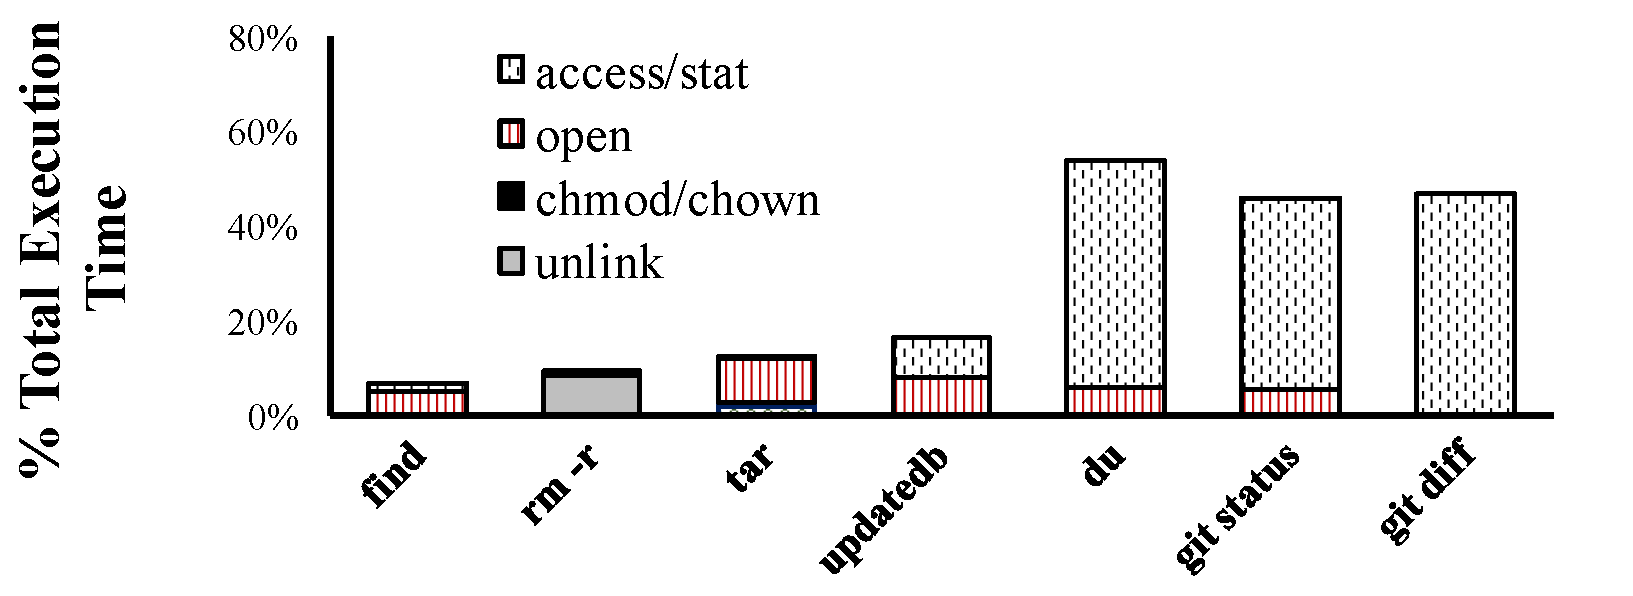
\includegraphics[width=5in]{dcache/plots/syscall-percentage.pdf} \\
\caption[Fraction of execution time on path-based system calls.]
{Fraction of execution time in several common utilities spent
executing path-based system calls with a warm cache, as measured with ftrace.}
\label{fig:dcache:lookup-frac}
%\vspace{-10pt}
\end{figure}

%\fixmedp{Please check these \% against time.  I think git diff is too high.  git status seems ok.}

Directory caches are essential for good application performance.
%Unix was designed such that ``(almost) everything is a file'',
%thus even accesses to in-memory file systems, device files, FIFOs and domain sockets
%first pass through the directory cache.
%In other words, 
Many common system calls must operate on file paths,
which require a directory cache lookup.
For instance, between 10--20\% of all system calls in the iBench system call traces do a path lookup~\citep{filenotafile}. 
Figure~\ref{fig:dcache:lookup-frac} lists the fraction of total execution time
%, as well as system time, 
several common command-line applications spend executing path-based system calls
(more details on these applications and the test machine in \S\ref{sec:dcache:eval}).
We note that these system calls include work other than path lookup,
and that these numbers include some instrumentation overhead;
% are coarse measurements that include  and work than path lookup;
%, and includes some time 
%for synchronous I/O (e.g., during {\tt rename}) as well as non-path tasks (e.g., creating 
%a file handle as part of {\tt open});
nonetheless, in all cases except {\tt rm},
the system call times and counts are dominated by
{\tt stat} and {\tt open}, for which 
%can be serviced from cache and for which 
path lookup is a significant component of execution time.
For these applications, path-based system calls account for 6--54\% of total execution time.
%and 25--77\% of system time.  
This implies that
lowering path lookup latency is
 one of the  biggest 
opportunities for a kernel to improve these applications' execution time.




\begin{figure}[t!]
\centering
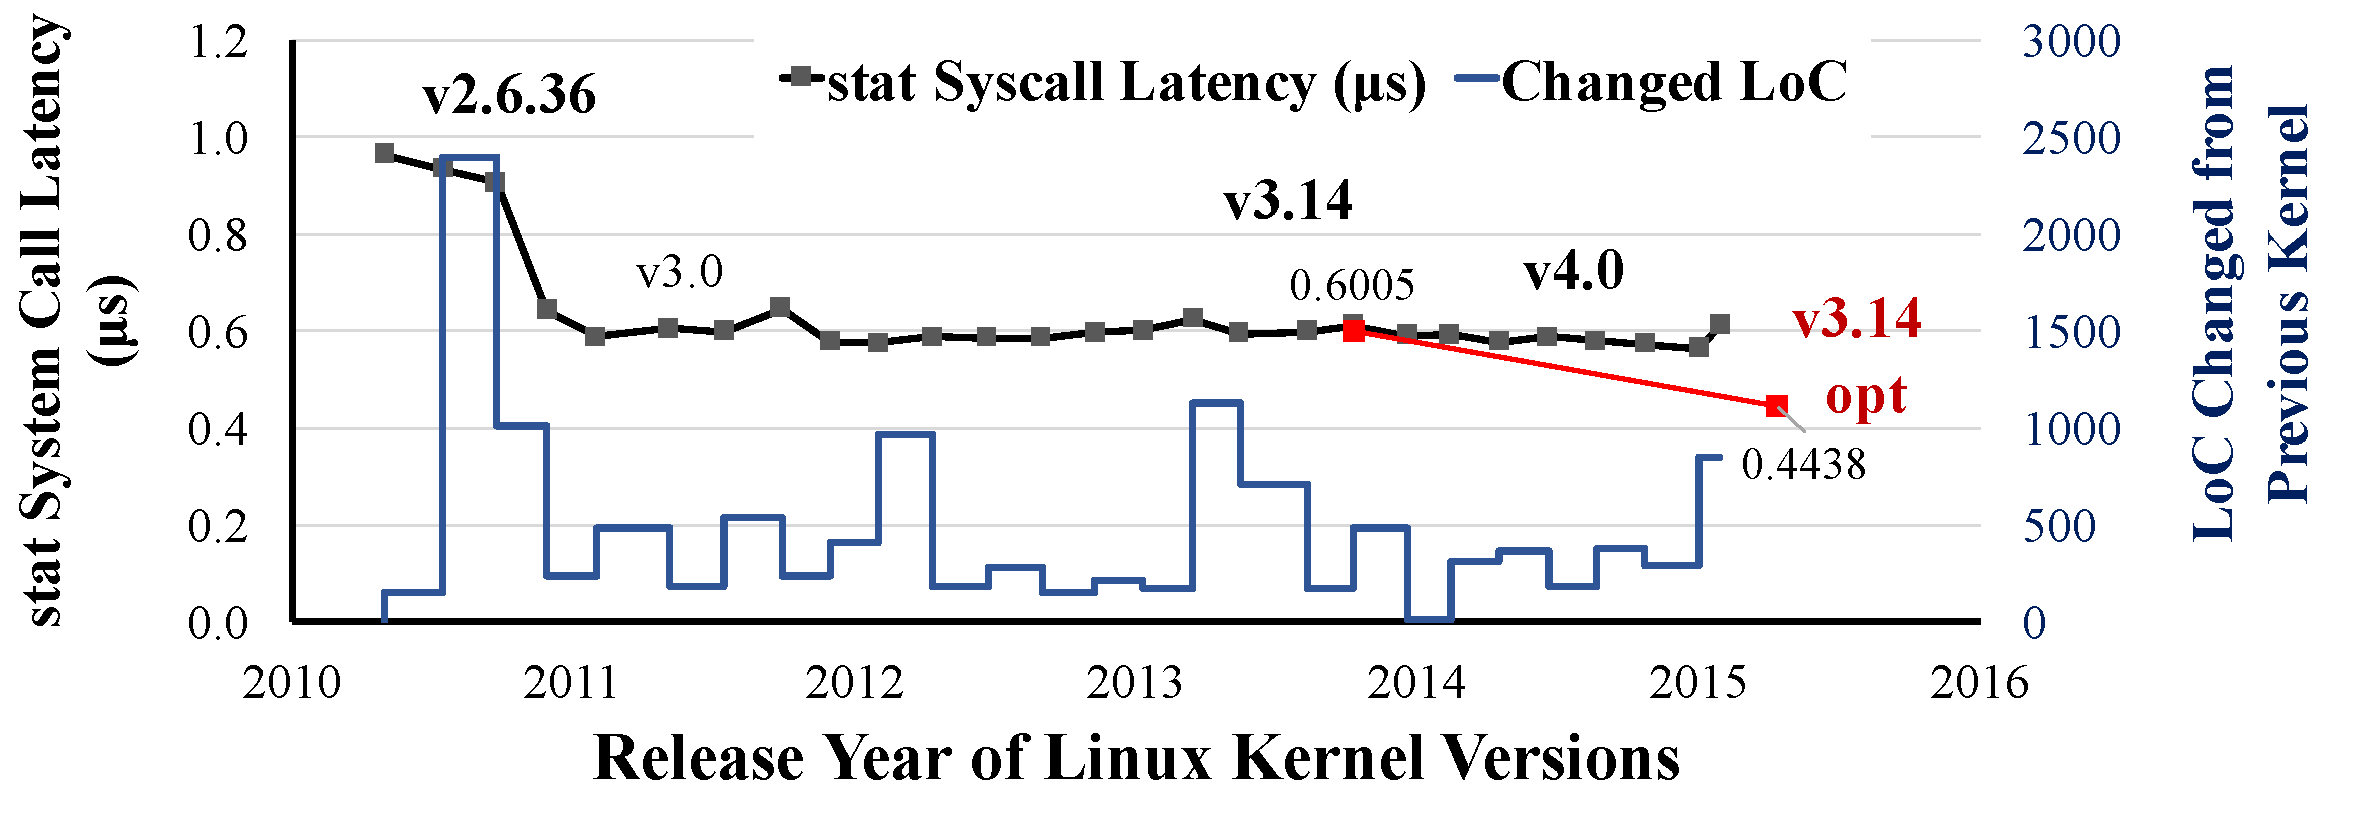
\includegraphics[width=6in]{dcache/plots/latency-by-version.pdf}
\footnotesize
\caption[Lantecy of {\tt stat} system call over years.]
{Latency of {\tt stat} system call with a long path {\tt XXX/YYY/ZZZ/AAA/BBB/CCC/DDD/FFF} on Linux over four years (lower is better), as well as the churn within the directory cache code (all insertions in {\tt dcache.c}, {\tt dcache.h}, {\tt namei.c}, {\tt namei.h} and {\tt namespace.c}). 
%Our optimizations significantly improve performance that has otherwise plateaued, despite significant ongoing developer effort.  
Our optimized \linuxver{} kernel 
further reduces {\tt stat} system call latency by \statspeedup{}\%.}
%\vspace{-15pt}
\label{fig:dcache:by-version}
\end{figure}


%\fixmedp{Add more evidence of lookup importance here: For instance, fraction of lookup time in file-related syscalls, or total lookup time in applications bound on file lookup latency.  }
Unfortunately, even directory cache hits are costly---0.3--1.1 \us{} for a {\tt stat} on our test Linux system, compared to only .04 $\mu$s for a {\tt getppid} and 0.3 \us{} for a 4 KB {\tt pread}. 
%\fixmetsai{Don, check this, I think read will be a better example, getppid is too trivial.}
This issue is taken particularly seriously in the Linux kernel community, which has 
made substantial revisions and increasingly elaborate optimizations to reduce the hit cost
of its directory cache, such as removing locks from the read path or replacing lock ordering with deadlock avoidance in a retry loop~\citep{corbet09jls,dcache-rcu}.
Figure~\ref{fig:dcache:by-version} plots directory cache hit latency against  lines of directory cache code changed 
over several versions of Linux, using a path-to-inode lookup \microbench{} on the test system described
in \S~\ref{sec:dcache:eval}.
These efforts have improved hit latency by 47\% from 2011 to 2013, but have plateaued
for the last three years.
%\fixmedp{if time, filter irrelevant changes from code deltas}
%at the cost of substantial developer effort.
%This latency appears to have plateaued 

The root of the problem is that the POSIX path permission semantics
seemingly require work that is linear in the number of path components,
and severely limit the kernel developer's implementation options.
%The root of this problem is that current directory cache
%designs reflect a straightforward implementation of the POSIX specification,
%which would seemingly require work that is linear in the number of path components.
For instance, in order to open file {\tt /\fnone{}/\fntwo{}/\fnthree{}} 
%for reading, 
one must have search permission
to parent directories {\tt /}, {\tt /\fnone{}}, and {\tt /\fnone{}/\fntwo{}},
as well as permission to access file {\tt \fnthree{}}.
The Linux implementation %of this specification is straightforward, 
simply walks the directory
tree top-down to check permissions.  
Unfortunately, when the critical path is dominated by 
walking a pointer-based data structure, 
including memory barriers on some architectures for multi-core consistency, 
modern CPUs end up stalling on hard-to-prefetch loads.
Moreover, because so many Linux features are built around this behavior, such as Linux Security Modules (LSMs)~\citep{wright+lsm},
namespaces, and mount aliases, it is not clear that any data-structural enhancements
are possible without breaking backward-compatibility with other Linux kernel features.
A priori, it is not obvious that a faster lookup algorithm, such as a single hash table lookup, 
can meet these API specifications and kernel-internal requirements; to our knowledge,
no one has tried previously.

%This paper proposes a decomposition of the directory cache, which allows
%most lookup operations to execute with a single hash table lookup (\S\ref{sec:dcache:dcache}),
%as well as optimizations to reduce the miss rate based on information that is {\em already in the cache}, but not used effectively (\S\ref{sec:dcache:readdir}).
%Our design maintains compatibility (\S\ref{sec:dcache:generalize}) through 
%several essential insights, including 
%how to separate the indexing of paths from checking parent permissions,
%and how to effectively and safely memoize the results of access control checks.


%% This paper proposes several new ways to organize a directory cache, which can yield 
%% substantial performance improvements over the current state of the art.
%% %This paper demonstrates that, despite this developer effort, there is still a substantial 
%% %missed opportunity hiding behind historical, intuitive, but not fundamental design choices.
%% Most of the Linux directory cache design reflects a straightforward implementation of the POSIX 
%% specification. %, with a division of labor that is suitable for mainstream file systems.

%This paper presents an alternative directory cache organization, which 
%improves performance by separating logical tasks, such as separating path indexing from permission checking; yet the design is sufficient to retain compatibility with POSIX.
%In the case of path lookup, 
%this paper demonstrates how 
%a per-component tree walk can be replaced with a single hash table lookup (\S\ref{sec:dcache:dcache}).
% without violating POSIX compliance.

%Our optimizations improve the performance of frequent lookup operations, but 
%introduce several costs, described in \S\ref{sec:dcache:dcache} and measured in \S\ref{sec:dcache:eval},
%which  we believe are acceptable and a net improvement for applications.
%First, these optimizations slow down infrequent modifications to the directory hierarchy, such as {\tt rename}, {\tt chmod},
% and {\tt chown} of a directory. 
%However, these slower operations
%account for less than .01\% of the system calls in the iBench traces~\citep{filenotafile}.
%Second,  the memory overheads of the dcache are increased.
%%(45\% per \dentry{}, as well as some  in our prototype).
%%(\fixmedp{XX MB} in our tests).  
%Third, lookup has a 
%probability of error from signature collisions that can be adjusted to be negligible
%%($2^{-141}$ in our configuration), 
%and within acceptable thresholds widely used by data deduplication systems~\citep{Debnath:2010:CSU:1855840.1855856, Srinivasan:2012:ILI:2208461.2208485, Quinlan:2002:VNA:645371.651321, Zhu:2008:ADB:1364813.1364831}.
%%, as well as how to remove
%%all memory barriers from the lookup path (\S\ref{sec:dcache:update}).
%In the micro-benchmark of Figure~\ref{fig:dcache:by-version}, our directory cache 
%optimizations improve lookup latency by 
%%revisions improve latency of accessing a long path
%%by 
%\statspeedup{}\% over unmodified Linux.
%%Our design addresses other missed
%%opportunities, such as identifying new opportunities to reduce the miss rate
%%through caching directory completeness.
%%\fixmedp{Do we want to highlight LoC?  3K is more than anything in the graph} \fixmetsai{Probably just mention in the evaluation. It's a metric that we should provide, but it's not awfully interesting.}
%%The total lines of code changed are fewer than 3,000 out of \fixmedp{XX}.
%%\fixmedp{Can we get 
%%, yet changes fewer than 3,000 lines of code.

%% SOSP cut - kind of long-winded
\begin{comment}
This paper rethinks current Linux directory cache design choices in light of the following goals:
\begin{compactitem}
\item {\bf Minimize the cost of a cache hit.} (\S\ref{sec:dcache:dcache}).
This means maximizing the benefit of temporal locality for frequent operations,
while pushing extra work of consistency maintenance onto less frequent, already-expensive operations.
%such as handling cache miss or updating massive metadata,
%in order to improve very frequent operations.
\item {\bf Maintain legacy compatibility.} (\S\ref{sec:dcache:generalize}).  Unix path semantics are complex, required by applications, file systems, and security modules, frustrating otherwise straightforward optimizations.  However tempting it may be to redesign path behavior to facilitate caching, path operations must exhibit the same behavior, with lower latency.
\item {\bf Never miss the same request twice in quick succession.} (\S\ref{sec:dcache:readdir}).  A number of less-frequent operations, such as reading a directory or secure temporary file creation, always miss in the cache {\em even if enough information is in cache to satisfy the operation.}  
%Of course, infrequent accesses should still be subject to a cache replacement policy, such as LRU.
\end{compactitem}
%Although directory caches must implement more complex semantics than a hardware memory cache,
%these principles should seem familiar to the reader with a basic architecture background.
%sadly, the Linux directory cache design violates all three.
\end{comment}

%This paper introduces several techniques to improve the performance of a directory cache,
%This paper explains several practical directory cache optimizations,
This paper demonstrates that these techniques improve performance for applications that use the directory cache heavily,
and the harm is minimal to applications that do not benefit.
%and that the worst case \microbench{} is only 12\% slower within \fixmedp{XX}\% of unmodified Linux.
%Each optimization we describe improves performance in isolation, and all can be combined.
%These optimizations change very few lines of code, and are backward-compatible with 
%legacy applications.  
%These changes are encapsulated in the VFS---individual file systems do not have to change their code.
%This paper describes a  prototype of these improvements implemented in Linux \linuxver{}.
%\S~\ref{sec:dcache:background} explains that the directory cache structure of Mac OS X, FreeBSD, and Solaris 
%are sufficiently similar that these principles should generalize.
%we compare and contrast Linux's directory cache
%with Mac OS X, FreeBSD, and Solaris in \S\ref{sec:dcache:background}, and explain inline how each
%optimization could be generalized to these other OS kernels.





%% \item {\bf Modularization and stackability}:
%% Any changes or optimizations must be implemented as modules inside Linux's VFS,
%% and can be stacked on top of the original design or any future optimizations. 
%% \item {\bf Backward compatibility}:
%% Any changes or optimizations must maintain least requirement of modifying any
%% file systems.
%% \item {\bf Generalization to other OSes}: Any changes or optimizations must be portable to other OSes with reasonable effort and change of design.




%% \dcache{} is proven to be effective on improving storage performance.
%% Experiments shows that,
%% in a Linux 3.x kernel, a \dcache{} with a xxx\% hit rate can speed up
%% metadata lookup and fetching time by xxx times.
%% \fixmetsai{experiment result, Linux version, and fs specs here}
%% However, we observed that Linux maintainers have made
%% constant and non-trivial efforts to improve \dcache{} in the Linux kernel.
%% We studied all \dcache{}-related source files in the Linux kernel Git repository,
%% and discovered that maintainers have committed
%% on average xxx revisions per source files.

%% We tested metadata lookup time on primary \dcache{}-related revisions.
%% Most changes on \dcache{} system only create xxx\%-xxx\% speed-up
%% than their predecessor.
%% \fixmetsai{result and graph here}.
%% Moreover, improvement to \dcache{} is still work-in-progress
%% for Linux maintainers.
%% \fixmetsai{reference to threads for latest dcache discussions}. 
%% All the evidences show that,
%% despite of significant reduction of storage operations,
%% efficiency of \dcache{} system internally still remains as a concern.

%% We argue that the design of \dcache{} needs to be carefully re-examined,
%% to fundamentally identify any missed opportunities that
%% improve value of \dcache{}.
%% At a high level, most optimization works for \dcache{} are focused on
%% improving ``how to cache'',
%% but we want to also lay eyes on ``what to cache'',
%% to ensure any valuable information returned from file systems
%% be captured by \dcache{} system.

%The contributions of this paper are as follows:
%\begin{compactitem}
%\item A performance analysis of the costs of path lookup and the opportunities
%to improve cache hit latency.
%\item A directory cache design that improves path lookup latency with a combination of techniques, including:
%  \begin{compactitem}
%  \item Indexing the directory cache by full path, reducing average-case lookup from linear to constant in the number of path components.
%  \item A Prefix Check Cache (PCC) that separates permission checking from path caching.  The PCC memoizes permission checks, and is compatible with LSMs~\citep{wright+lsm}.
%  \item Reducing the cost of checking for hash bucket collisions with path signatures.
%  \end{compactitem}
%\item Identifying opportunities to leverage metadata the kernel already has to reduce miss rates, such as tracking whether a directory is completely in cache.
%\item Carefully addressing numerous, subtle edge cases that would frustrate rote application of these techniques, such as integration with symbolic links and Linux namespaces.
%\item A thorough evaluation of these optimizations.  For instance, our optimizations improve throughput
%of the Dovecot IMAP server by up to \dovecotspeedup\% and latency of 
%updatedb by up to \updatedbspeedup{}\%.
%%git version control system by up to 25\%.
%
%\end{compactitem}

\subsection{Stream I/O}
\label{sec:abi:streams}



\issuedone{1.2.a}{discuss resource management at host level (I/O)}
I/O is part of the foundation
of an OS, to allow an application to interact with
other machines, users, applications, or system software.
An OS typically supports three types of I/O:
%An application requires interaction with the world during its execution, using I/O devices.
%I/O is a common feature of almost every OSes.
%The typical I/O needed in an application
%can be catagorized into three types:
{\bf storage}, for externalizing data to a permanent store;
{\bf network}, for exchanging data with another machine over internet;
and {\bf RPC} (remote procedure call),
for connecting concurrent applications or processes.
An OS must contain features for all three types of I/O abstractions,
and manages the resources on I/O devices, such as hard drives and NICs (network interface controllers).
Therefore, unless an I/O device is virtualized and dedicated to
an application or a guest,
a host OS must take a major role in I/O management;
for the least, a host OS has to share the resources among multiple applications or guests,
and contain the drivers to interface with the I/O devices.




%externalizing data to outside of the machines (i.e., networking);
% (i.e., storage);
%and  (i.e., remote-procedure call).
%A modern OS may define several abstractions
%for each types of I/O; for example, a file in Linux can be read using several system calls,
%including \syscall{read}, \syscall{pread}, and \syscall{readv};
%RPC in Linux is based on multiple inter-process abstractions,
%including pipes, UNIX sockets, and signals.




\fixmedp{Perhaps you want to start with defining a single byte stream abstraction? And then talk about how different URIs leads to different subclasses?}
The basic I/O abstraction in the host ABI
is a simple byte stream.
A byte stream allows sending or receiving information over an I/O device
as a continuous byte sequence.
According the type of I/O, a byte stream is restructured as the I/O device demands;
for example, on a storage device,
a byte stream is logically stored as a sequential file,
but physically divided into blocks;
on a NIC, a byte stream is transfered as packets, and identified by IP address and port number bound to a network socket;
a RPC stream can be simply a FIFO (first-in-first-out),
which applications or processes use to pass messages.
The host ABI for I/O is similar to the API of a UNIX-style OS,
which treats ``everything as a file descriptor''
and allows utilizing different types of I/O devices through the same file system APIs, including \syscall{read} and \syscall{write}.
Managing I/O as byte streams simplifies the development of both the library OS and PALs.
%The host ABI includes \hostapis{} for single-flavored, stream-type I/O, similar to the API of a UNIX-style OS.
%In general, a UNIX-style OS
%follows the design where ,
%meaning that each I/O abstraction is encapsulated by the file system APIs, such as \syscall{read} and \syscall{write}, to send and receive data on a file, a network socket, or a FIFO (first-in-first-out).
%but categorizes into three types:
%{\bf network connections}, {\bf regular files}, and {\bf RPC streams}.


The host ABI identifies I/O streams by URIs (unified resource identifier).
%These I/O streams
%are created or connected using a URI (unified resource identifier),
A URI is a unique name which describes 
both the subclass of an I/O stream, and the information for locating or identifying an I/O stream on an I/O device or inside the host OS.
The subclass of an I/O stream is identified by the URI prefix,
a keyword that represents different types of I/O: ``\palkeyword{file:}'' for regular files; ``\palkeyword{tcp:}'' and ``\palkeyword{udp:}'' for network connections; and ``\code{pipe:}'' for RPC streams.
The rest of the URI represents an identifier of the I/O stream:
for example, a file can be identified by a path located in a hierachical file system;
a network connection can be identified by the socket address.
The URIs standardize the way of identifying I/O resources inside various host OSes.


%According to the prefix of URI,
%the PAL can create either a synchronous I/O stream (e.g., a file or a connected socket)
%or named I/O server (e.g., a listening TCP socket).
%Modern OSes contain several out-of-band or asynchronous I/O abstractions, to improve the latency or CPU idle time
%when polling I/O streams.
%Although using out-of-band or asynchronous I/O is beneficial for application performance,
%providing these I/O features can be challenging for a host.
%Therefore, in \graphene{}, the host ABI restricts I/O abstractions to only synchronous stream I/O.


\fixmedp{Define these semantics without a reference to POSIX, so that the document is self-contained.}
The \hostapis{} defined in the host ABI for I/O are as follows:
%The host ABI for stream I/O presents a simplified, {\b POSIX file system}.
%A POSIX file system
%encapsulates I/O abstractions,
%including files, sockets, pipes, and even character devices,
%in the file system API.
%The host ABI contains several functions
%which resemble the POSIX API:
\palcall{StreamOpen} creates or opens an I/O stream;
\palcall{StreamRead} and \palcall{StreamWrite}
send and receive data over an opened I/O stream;
%are similar to \syscall{open}, \syscall{read}, and \syscall{write} in behavior, with a simplified, explicit semantic;
\palcall{StreamMap} maps %a is equivalent to \syscall{mmap} with a \code{MAP\_FILE} flag, mapping
a regular file to the application's memory; %, for reading or writing data.
\palcall{StreamAttrQuery} and \palcall{StreamAttrQuerybyHandle}
retrieves the file metadata and I/O attributes;
%as \syscall{stat} and \syscall{fstat} do;
%The POSIX-style functions simplify the porting of the host ABI
%on hosts with a similar specification.
\palcall{StreamWaitForClient} blocks and creates an I/O stream for incoming network or RPC connection;
\palcall{StreamSetLength} truncates a regular file;
\palcall{StreamFlush} clears the I/O buffer inside the host OS.
The following sections will discuss these \hostapis{} in details.





\subsubsection*{Opening or creating an I/O stream}




\begin{paldef}
HANDLE StreamOpen (const char *stream_uri,
                   u16 access_flags, u16 share_flags,
                   u16 create_flags, u16 options);
\end{paldef}



\palcall{StreamOpen} opens an I/O stream, % for future operations,
according to a URI given by \palkeyword{stream_uri} as a string argument. % to identifies resources associated with the I/O stream. 
The specification of 
\palcall{StreamOpen} includes interpreting the URI prefixes and syntaxes of \palkeyword{stream_uri},
and allocating the associated resources in the host OS and on the I/O devices.
\fixmedp{The term ``Opaque pointer'' is useful here}
If \palcall{StreamOpen} succeeds, it returns a {\bf stream handle}.
A stream handle is stored by the guest as an identifier to the opened I/O stream.
A stream handle is an opauqe pointer, which means the guest should only reference it as an identifier, and never try to interpret the content.
On the other hand, if \palcall{StreamOpen} fails (e.g., invalid arguments or permission denied), it returns a null pointer with the failure reason delivered with an exception.
% A stream handle is similar to a file descriptor in the POSIX API,
%but defined as a pointer to a data structure containing the stream information.
%The internal structure of a stream handle is up to the I/O stream type and the implementation of each PAL;
%a library OS is supposed to reference a stream handle
%only as an identifier.


\fixmedp{Need a listing of all the values of flags}
Other arguments of \palcall{StreamOpen} specify the options for opening an I/O stream:

\begin{compactitem}

\item
\palkeyword{access_flags} specifies the access mode of the I/O stream, which can be either \palkeyword{RDONLY} (read-only), \palkeyword{WRONLY} (write-only), \palkeyword{APPEND} (append-only), and \palkeyword{RDWR} (readable-writable).
The first three access modes are only available
for regular files; if the opened stream is a network or RPC stream, the access mode is always \palkeyword{RDWR}.
The access modes specify the basic access permissions that an application can request when opening a file.
The access permissions are validated by the host OS, based on user configurations.
For example, a file configured as append-only for the running application can only be opened in the \palkeyword{APPEND} mode.

\item
\palkeyword{share_flags} specifies the permissions for sharing a regular file (ignored for other types of  I/O streams)
with other applications, either in \graphene{} or in the host OS.
\palkeyword{share_flags} can be a combination of six different values:
\palkeyword{OWNER_R}, \palkeyword{OWNER_W}, and \palkeyword{OWNER_X}
represent the permissions to be read, writed, and executed by the creater of the file;
\palkeyword{OTHER_R}, \palkeyword{OTHER_W}, and \palkeyword{OTHER_X}
represent the permissions to be read, writed, and executed by everyone else.
The permissions are externalized to the host file system; access modes given in future execution are validated against the permissions.

\item
\palkeyword{create_flags} specifies whether to create a regular file,
when it does not exist in the host file system.
If \palkeyword{create_flags} is given as \palkeyword{TRY_CREATE},
it creates the file no matter if the file exists.
If \palkeyword{create_flags} is given as \palkeyword{ALWAYS_CREATE},
it fails if the file already exists.

\item
\palkeyword{options} specifies a set of miscellaneous options to configure the opened I/O stream.
Currently \palcall{StreamOpen} only accepts one option: \palkeyword{NONBLOCK} specifies that the I/O stream will never block whenever the guest attempts to read or write data.
The nonblocking I/O option is necessary for performing asynchronous I/O in the guest, to overlap the blocking time of multiple streams by polling (using \palcall{ObjectsWaitAny}).

\end{compactitem}


%includes different syntaxes for interpreting the URI and the rest of arguments,
%and different behaviors for creating or opening an I/O stream,
%according to the URI prefixes.
%uses a URI (uniform resource identifier), for specifying the I/O stream.
%An URI identifies both the type of I/O and the distination or location of the I/O stream.
%The type of a I/O stream is determined by URI prefix.
According to the consecutive operations, \palcall{StreamOpen}
returns two types of handles: One type represents a simple byte stream;
the other type is a server handle, which can wait on remote clients to initiate handshakes
for creating a byte-stream connection.
A server handle can be bound as a network server or a RPC server.
Because a server handle is not a byte stream, it cannot be directly read or written,
but can be given to \palcall{ServerWaitForClient} to block and receive a client connection.
The host ABI includes the abstraction of creating server handles
because receiving client connections requires control at the TCP/IP layer
and allocating host resources,
which cannot be implemented in the guest unless
the network stack is virtualized.




\palcall{StreamOpen} accepts the following URI prefixes and syntaxes for creating a byte stream or a server handle:


\begin{compactitem}

\item \palkeyword{file:[path]} creates or opens a regular file on the host file system.
The opened file is located by a path---either an absolute path from the root of the host file system, 
or a relative path.
\fixmedp{Mention CWD is relative to where the app is launched from. It may also be worth noting that this is included for convenience, but there are some security risks to using relative paths.}
A relative path is located from the initial directory where the application is launched,
and will never change afterward.
\palcall{StreamOpen} accepts relative paths for the convenience of locating application files packaged and shipped together.
Note that there could be security concerns
that a relative path may collide with another absolute path, or be ambiguous if the path starts with a ``dot-dot'' (i.e., walking back a directory).
Fortunately, both cases can be checked by the guest, as long as
the initial directory is specified by the host.
%based on user configurations.

\item \palkeyword{tcp:[address]:[port]} or \palkeyword{udp:[address]:[port]} creates a TCP or UDP connection to a remote server,
based on the IPv4 or IPv6 address and port number of the remote end.
One a connection is created,
it will exists until it is torn down by both sides.

\item \palkeyword{tcp.srv:[address]:[port]} or \palkeyword{udp.srv:[address]:[port]} create a TCP or UDP server handle which can receive remote client connections.
A TCP or UDP server is bound on a IPv4 or IPv6 address and an idle port number.
If the specified port number is smaller than 1024,
it may require additional privilege from the host OS.

\item \palkeyword{pipe.srv:[name]} or \palkeyword{pipe:[name]} create a named RPC server or a connection to a RPC server.
The name of a RPC server is an arbitrary, unique string.
An RPC stream is an efficient way for passing messages between applications or processes
running on the same host,
compare with using a network stream locally.
An RPC stream is supposed to be low-latency, and can scale up to significantly
more concurrent connections
than the limitation on network streams.

%The stream can be either a server which awaits incoming connection from other processes,
%or a client to an existing server.

\end{compactitem}



%Besides the abstraction,
%\palcall{StreamOpen}
%also inherits similar definitions of function arguments,
%including \palkeyword{access_flags}, \palkeyword{share_flags}, \palkeyword{create_flags}, and \palkeyword{options},
%from the POSIX-style \syscall{open}.
%%also inherit similar meanings from the options of \syscall{open}.
%These arguments specify the access type, file permission, creation mode, and other miscellaneous options of the I/O streams:
%for example, the access type can be specified as readable or writable,
%and the creation mode can be either explicit or implicit.
%An important concern is the choice of file permission (specified by \palkeyword{share_flags}), since the host ABI does not expose user credentials
%from the host.
%Setting the file permission in the host
%is mostly a usability feature: 
%an application can run more smoothly if some file permissions are externalized.
%For example, a compilor can create an executable with the execution permission, so that the consecutive building script can run the executable.
%The host ABI also externalizes the file permission
%which specifies specify whether a file can be shared with other applications.


\palcall{StreamOpen} defines the scope of enforcing and configuring security isolation in the hosts.
%URIs for \palcall{StreamOpen} represent three types of 
The host ABI restricts the sharing of host resources
to type types of simple I/O streams (i.e., file, network, and RPC). 
Other host resources, such as threads and memory,
are local to each process, and thus can be isolated by dedicating the host resources.
%Restricting the shareable host resource to I/O streams simplifies
%the enforcement of security policies in the hosts.
Therefore, in the host ABI, \palcall{StreamOpen} is the only \hostapi{}
which requires permission checks in the hosts.
Moreover, a user can configure the policies of sharing I/O streams by
whitelisting the URIs that are permitted for an application.





\subsubsection*{Reading or writing an I/O stream}



\begin{paldef}
u64 StreamRead  (HANDLE stream_handle, u64 offset,
                 u64 size, void *buffer);
u64 StreamWrite (HANDLE stream_handle, u64 offset,
                 u64 size, const void *buffer);
\end{paldef}                   
              
\palcall{StreamRead} and \palcall{StreamWrite} synchronously
read and write data over an opened I/O stream.
Both \hostapis{} receive four arguments: a \palkeyword{stream_handle} for referencing the target I/O stream;
\palkeyword{offset} from the beginning of a regular file
(ignored if the stream is a network or RPC stream);
\palkeyword{size} for specifying how many bytes are expected to be read or written;
and finally, a \palkeyword{buffer} for storing the read or written data.
At success, the \hostapis{} return the number of bytes
actually being read or written.


     




%The host ABI features include synchronously reading and writing data over an I/O stream.
%The behavior of \palcall{StreamRead} and \palcall{StreamWrite} is slightly different between a file stream and other type of stream:
%when reading or writing a file stream, \palcall{StreamRead} and \palcall{StreamWrite} accesses the file at a specific offset from the beginning of the file;
%otherwise, when accessing a network or RPC stream,
%the argument \palkeyword{offset} is ignored, and thus the ABI works similar to \syscall{read} and \syscall{write}.



\palcall{StreamRead} and \palcall{StreamWrite} avoid the semantics of sequential file access
to skip the migration of stream handles.
A regular file opened by \palcall{StreamOpen} (not in the append-only mode)
can only be read or written at an absolute offset
from the beginning of the file.
The random file access prevents the host OSes to track the offset
as an internal state,
and allows a migrated guest to reopen the I/O stream on another host
without migrating the host OS states.
Because all the host OS states associated with an I/O stream is only meaningful to the host,
and can be receated anytime,
the I/O stream appears to be {\em stateless} to the guest.



%The design is to keep the stream handle stateless inside the PAL,
%for cleanly migrating a library OS.
%Since the library OS is responsible of maintaining the offset of a file descriptor,
%a library OS instance can be easily detach from a PAL,
%by simply ``invalidating'' a stream handle;
%the library OS should be able to always reopen the stream after migration,
%or after a failure of accessing a stream handle,
%to recover the state of an I/O stream.



The host ABI does not includes asynchronous I/O semantics, or peeking into network or RPC buffers inside the host OS.
%Another challenge in the library OS, regarding I/O streams,
%is to support asynchronously I/O, or peeping data received over a network or RPC stream.
%This design decision is made to keep the host ABI simple.
Asynchronous I/O and peeking the buffers are both
common OS features that an application may depend on.
Although the features are not included in the host ABI,
the guest (i.e., the \libos{}) is supposed to emulate these features using the synchronous \palcall{StreamRead} and \palcall{StreamWrite},
combined with other \hostapis{} (e.g., \palcall{ObjectsWaitAny})
to prevent blocking on an I/O stream.
The guest can also allocate its own buffer to store data prematurely received from an I/O stream,
to serve the buffer peeking feature.
More details of these features are discussed in Chapter~\ref{chap:libos}.

%To implement the full Linux I/O features,
%the library OS must emulate asynchronous I/O,
%using the synchronous
%\palcall{StreamRead} and \palcall{StreamWrite}.
%The emulation requires opening the I/O stream in a non-blocking mode,
%and polling the stream handle before reading or writing data.
%The library OS can also buffer the data being read or written over a stream,
%as long as the buffered state is coordinated over every processes
%which share the same stream.


\paragraph{Alternative.}
An alternative strategy is to define a host ABI with asynchronous I/O semantics.
An asynchronous read or write
does not return a result immediately; instead, it creates an event handle
which can be polled arbitrarily.
An ABI that asynchronously reads and writes an I/O stream
potentially has more predictable semantics,
because the guest can explicitly tell which \hostapis{} will be blocking.
This strategy
is taken by Bascule~\cite{baumann13bascule}.
\graphene{} chooses synchronous I/O over asynchronous I/O in the current host ABI,
because synchronous I/O is a more common feature in host OSes.


 


%Defining  \hostapis{} for asynchronous read and write
%may potentially sacrifice portability, \fixme{cites some host that doesn't have async IO}
%since asynchronous I/O is less common seen in OSes.
%However, 
%can potentially be a more flexible option for emulating other I/O features in the guest.
%For example, the guest can emulate a synchronous read by polling a stream followed by asynchronously reading it.



%An asynchronous I/O ABI can be potentially
%more flexible for implementing the library OS features,
%as it can emulate both synchronous and asynchronous behaviors
%without buffering.
%The only reason that we choose synchronous over asynchronous I/O
%in the host ABI is to reduce the porting effort,
%especially for a host which lacks
%asynchronous I/O features.



\subsubsection*{Mapping a file to memory}
                   
\begin{paldef}            
u64 StreamMap (HANDLE stream_handle, u64 expect_addr,
               u16 protect_flags, u64 offset, u64 size);
\end{paldef}


\palcall{StreamMap} maps a file stream to an address in memory, for reading and writing data, or executing code stored in a binary file.
\palcall{StreamMap} creates a memory region
as either a copy of the file,
or a pass-through mapping which shares file updates with other processes.
When calling \palcall{StreamMap},
the guest specifies an expected address in memory for mapping the file, or a null address (i.e., zero) for mapping at a random address decided by the host.
\palkeyword{expect_addr}, \palkeyword{offset}, and \palkeyword{size} have to be aligned
with the allocation granularity of the hosts (more discussion in Section~\ref{sec:abi:memory}).
\palkeyword{protect_flags} specifies the protection mode
of the memory mapping, as a combination of \palkeyword{READ} (readable), \palkeyword{WRITE} (writable), \palkeyword{EXEC} (executable), and \palkeyword{WRITE_COPY} (writable local copy).
At success, \palcall{StreamMap} returns the starting address of the mapped area; otherwise, a null address is returned.




The host ABI includes \palcall{StreamMap} for two reasons. First, memory-mapped I/O is suitable for certain file access patterns of applications, and cannot be fully emulated by the guest using \palcall{StreamRead} and \palcall{StreamWrite}.
An application often chooses memory-mapped I/O for
avoiding the overhead of memory copy and context switch, %, especially when the application contains
for frequent, small, random file reads and writes.
Second, memory-mapped I/O is asynchronous by nature.
The data written to a file-backed memory mapping can be lazily flushed out to the storage;
the same feature is difficult to emulate in the guest
%due to lack of ability to efficiently determine which pages are recently updated,
% and thus should be synchronized with the storage.
without an efficient way of marking recently-updated pages (page table dirty bits can only be accessed in host OSes).
%without access to dirty bits in the page table.




%However, the challenge to implementing this behavior
%is to externalize the latest file state
%written by the application,
%on a host which disallows file-backed memory.
%For example, in a SGX enclave, all memory will have to be private memory,
%to be individually encrypted by the CPU.
%For a host which doesn't support pass-through file mappings,
%\palcall{StreamMap}
%can only guarantee writing out
%the latest file state to the disk when the memory is unmapped, using \palcall{VirtMemFree}.


\fixmedp{there should be an explicit semantics about when the mapping is visible back to the host, like on a sync, with the option to flush earlier}
Although \palcall{StreamMap} allows multiple processes to map the same file into memory, it does not guarantee the data to be coherently shared across processes.
Because memory-mapped I/O is asynchronous,
the data written in the memory is only guaranteed to be flushed to the storage
when the memory mapping is unmapped.
Also, the host ABI drops the assumption of memory sharing, especially for an isolated environment like SGX.
It is optional for the host to flush earlier,
or to coherently share the memory across multiple processes.













\subsubsection*{Listening on a server}


\begin{paldef}
HANDLE ServerWaitforClient (HANDLE server_handle);
\end{paldef} 


\palcall{ServerWaitforClient} waits on a network or RPC server handle, %created with a URI that starts with \palkeyword{tcp.srv:}, \palkeyword{udp.srv:}, or \palkeyword{pipe.srv:},
to receive an incoming client connection.
%Besides the I/O streams which can be directly read or written,
%the host ABI also supports creation
%of I/O stream server, which can be
%connected from another process (to a RPC stream server), or another host (to a network server), as a client of the server.
A network or RPC server handle cannot be accessed by \palcall{StreamWrite} or \palcall{StreamRead};
instead, the host OS listens on the server handle,
and negotiates the handshakes for incoming connections.
Once a connection is fully established,
the host OS returns a client stream handle, which can be read or written as a simple byte stream.
Before any connection arrives, \palcall{ServerWaitforClient} blocks eternally.
if a connection arrives before the guest calls \palcall{ServerWaitforClient},
the host can optionally buffer the connection in a limited backlog; the maximal size of server backlogs is up to the user configurations. The host will drop incoming connections when the backlog is full.




%I/O stream server has to block until a client
%connects the server, using \palcall{StreamWaitForClient}.
%\palcall{StreamWaitForClient} will return a stream handle, which represents a connection with the client.
%Other implementation
%is up to the host: for example,
%the host may decide a maximal number of incoming connections to buffer.









\subsubsection*{File and stream attributes}

%The host ABI features also include retrieving the metadata of an I/O stream.
%The retrieval of metadata is not limited to files,
%but also network sockets and RPC streams. %, to query the information regarding the streams.
%An example of metadata is the address of a network stream;
%when an unbound network stream is created,
%the host will randomly bind the stream to a local, temporary port, for identifying the connection at the IP (internet protocol) level;
%the POSIX API
%reveals the local port number
%to the applications,
%using \syscall{getsockname}.
%Other stream metadata required by Linux or POSIX functionality
%includes the total bytes written over an I/O stream, and the permission to sharing an I/O stream with other applications.
%The host ABI includes two functions for querying stream metadata:

\begin{paldef}
bool StreamAttrQuerybyHandle (HANDLE stream_handle,
                              STREAM_ATTRS *attrs);
bool StreamAttrQuery (const char *stream_uri,
                      STREAM_ATTRS *attrs);

\end{paldef}

Both \palcall{StreamAttrQuerybyHandle} and \palcall{StreamAttrQuery} query the attributes of an I/O stream, and return the attributes in a \palkeyword{STREAM_ATTRS} data structure.
The only difference is that \palcall{StreamAttrQuerybyHandle} queries an opened stream handle,
whereas \palcall{StreamAttrQuery} queries a URI without opening the I/O stream.
\palcall{StreamAttrQuery} is convenient for querying stream attributes when the guest is not planning to access the data of an I/O stream.
%Because \palcall{StreamOpen} involves more operations in the host OS,
%\palcall{StreamAttrQuery} can quickly retrieve the attributes without actually opening the stream.
Both \hostapis{} return true or false for whether the stream attributes are retrieved successfully.



%Both functions fill out a data structure given by the library OS,
%with metadata regarding an I/O stream
%identified by either a stream handle or a URI.
%Keeping both functions can be convenient for the library OS to query a file without creating a stream handle;
%however, we can always consolidate the host ABI
%with only \palcall{StreamAttrQuerybyHandle},
%because \palcall{StreamAttrQuery} can be replaced by \palcall{StreamAttrQuerybyHandle}
%after \palcall{StreamOpen}.




\begin{paldef}
typedef struct {
    u16 stream_type, access_flags, share_flags, options;
    u64 stream_size;
    u64 recvbuf, recvtimeout;
    u64 sendbuf, sendtimeout;
    u64 lingertimeout;
    u16 network_options;
} STREAM_ATTRS;
\end{paldef}


The \palcall{STREAM_ATTRS} data structure consists of multiple fields specifying the attributes assigned to an I/O stream since creation.
\palkeyword{stream_type} specifies the type of I/O stream that the handle references to.
\palkeyword{access_flags}, \palkeyword{share_flags}, and \palkeyword{options} are the same attributes assigned to an I/O stream when the stream is created by \palcall{StreamOpen}.
\palkeyword{stream_size} has different meanings for files and network/RPC streams:
if the handle is a file, \palkeyword{stream_size} specifies the total size of the file;
if the handle is a network or RPC stream, \palkeyword{stream_size} specifies the size of pending data currently received and buffered in the host.


The remaining attributes are specific to network or RPC streams.
\palkeyword{recvbuf} and \palkeyword{sendbuf} specify the limitation of buffering the pending bytes, either inbound or outbound.
\palkeyword{recvtimeout} and \palkeyword{sendtimeout} specify the receiving or sending timeout (in microsends)
before a stream is considered being disconnected abruptly.
\palkeyword{lingertimeout} specify the timeout for closing or shutting down a connection
to wait for the pending outbound data.
\palkeyword{network_options} is a combination of flags that specify the options of configuring a network stream.
Currently \palkeyword{network_options} accepts the following generic options:
\palkeyword{KEEPALIVE} (enabling keep-alive messages), %\palkeyword{CORK} (don't send out partial data),
\palkeyword{TCP_NODELAY} (no delay on sending small data),
and \palkeyword{TCP_QUICKACK} (no delay on sending ACK responses).


\begin{paldef}
bool StreamAttrSetbyHandle (HANDLE stream_handle,
                            const STREAM_ATTRS *attrs);
\end{paldef}


\palcall{StreamAttrSetByHandle} is a \hostapi{} newly introduced by \graphene{}.
\palcall{StreamAttrSetByHandle} changes the attributes initially assigned to an I/O stream, and externalizes the change to the host OS.
\palcall{StreamAttrSetByHandle} is given an updated \palkeyword{STREAM_ATTRS} data structure,
which contains the new attributes to be assigned to the I/O stream.
\palkeyword{stream_type} cannot be changed, as well as any attributes that violate the limitation imposed by the host.


A dilemma for defining the \palkeyword{STREAM_ATTRS} data structure is
to decide which stream attributes,
especially for a network stream, should be exposed by the host,
A network stream attribute can be derived from an optional feature inside the host network stack,
or a configuration at the NIC level.
Exposing these stream attributes allows the guest to export APIs for applications
to fine-tune the I/O performance.
However, exposing too many attributes makes the host ABI
less portable on different host OSes, since these attributes may not have their equivalences in certain host OSes.
Eventually, a guest should not expect every attributes defined in \palkeyword{STREAM_ATTRS} to be always configurable,
and \palcall{StreamAttrSetByHandle} will raise a failure
if the guest tries to set an unavailable attribute.





%To complete the library OS implementation, \graphene{} introduces a new function,
%,
%for changing the metadata of an I/O stream.
%The main reason for changing metadata
%is to configure a network or RPC stream with several device-specific options,
%such as the number of lingering connections,
%or enabling the TCP keepalive feature.


%\subsubsection*{Truncating a file or flushing a stream}




%To externalize the change to an I/O stream, the library OS must ensure a file is truncated to the right length (\palcall{StreamSetLength}), or a network or RPC Stream has flushed the host buffer (\palcall{StreamFlush}).
%Both functions are private to a process; if multiple processes try
%to set the file length or flush a stream at the same time, one of the function calls may be ignored by the host.


\begin{paldef}
bool StreamSetLength (HANDLE stream_handle, u64 length);
\end{paldef}


Finally, \palcall{StreamSetLength} expands or truncates a file stream to a specific length.
In general, the data blocks on storage media are allocated dynamically
to a file when the file length grows.
If \palcall{StreamWrite} writes data beyond the end of a file, it automatically expands the file, by allocating new data blocks on the storage media.
However, a file-backed memory mapping created by \palcall{StreamMap}
lacks an explicit timing to expand the file
when writing to the memory mapped beyond the end of file.
\palcall{StreamSetLength} can explicitly request the host to expand a file to an appropriate length,
so that consecutive memory write will never raise memory faults.
\palcall{StreamSetLength} can also shrink a file to the actual data size
if the file has overallocated resources earlier.







%\subsection*{\graphene{}-specific stream I/O features}

%\begin{paldef}
%void StreamDelete (HANDLE stream_handle, uint direction);
%\end{paldef}


\paragraph{Listing a directory.}
\graphene{} extends the stream I/O feature in the host ABI to retrieve directory information.
A file system usually organizes files in directories,
and allows applications to retrieve a list of files in a given directory.
Instead of adding new \hostapis{} for directory operations,
the host ABI uses existing \hostapis{}, namely \palcall{StreamOpen} and \palcall{StreamRead},
for listing a directory.
When \palcall{StreamOpen} is given a file URI that points to a directory,
such as ``\code{file:/usr/bin}'',
\palcall{StreamOpen} returns a stream handle
which allows consecutive \palcall{StreamRead} calls to read the file list
as a simple stream.
The stream handle that references to a directory can only be read as FIFO (first-in-first-out),
and the returned data should contain a series of file names as null-terminated strings.
The stream handle cannot be written or mapped into memory.



%A POSIX file system contain a hierarchy of directories
%containing files and subdirectories.
%The file I/O in POSIX requires listing the entries in a directory;
%a POSIX function, \syscall{readdir}, returns a list of file and subdirectory names
%in a directory.
%In \graphene{}, we face a decision of whether to include directory I/O
%in the host ABI.
%An option is to maintain a local file in each directory
%to store a list of file and subdirectory names;
%however, this solution will requires maintaining the list whenever a new file or subdirectory is created.
%Therfore, we extend the host ABI,
%to allow opening a directory as a stream handle.
%The library OS can read a list of file and subdirectory names from a directory stream handle,
%generated by the hosts.




\paragraph{Character devices.}
The host ABI also supports reading or writing data over a character device, including a terminal.
A terminal can be connected as a stream handle,
using a special URI called \palkeyword{dev:tty}.
Other character devices include the debug stream of a process (the URI is \palkeyword{dev:debug}),
equivalent to writing to \code{stderr} in POSIX.





\subsection{Page management}
\label{sec:abi:memory}



%Linux applications 
%are generally developed and compiled under the assumption that the memory is managed
%by the OS with page-level granularity.
%%generally requires system API
%%for allocating, protecting, and deallocating memory at the same granularity.
%%A x86 application may require memory allocation to be strictly at the granularity of four-kilobyte pages,
%The primary Linux memory API,
%including \syscall{mmap}, \syscall{mprotect}, and \syscall{munmap},
%allows an application
%to arbitrarily create, modify, and destroy VMAs (virtual memory areas),
%wholly or partially,
%as long as the requested areas align to
%4KB.
%%Developers can avoid hard-coding the granularity in an application,
%%by retrieving the system setting using \syscall{getpagesize}.
%Specifically, the Linux dynamic loader (i.e., \code{ld.so}) %, an ubiqutous user-space component in Linux,
%uses \syscall{mmap} to map a binary file to a large memory area,
%and then divides the mapping into 4KB-aligned code and data segments.
%To implement the Linux memory API,
%the memory management scheme of the host ABI
%must be at least as fine-grained as 4KB pages.

\issuedone{1.2.a}{Discuss resource management at host level (pages)}
In the hos ABI, the abstraction for page management
is a {\bf virtaul memory area (VMA)}, a page-aligned, nonoverlaping region
in the guest's virtual address space.
A virtual memory area
specifies the memory region that requires the host OS to allocate the page resources,
either statically or dynamically.
There are two types of VMAs: one is a file-backed VMA, which is created by \palcall{StreamMap} and backs the memory pages with file data blocks.
The other type is an anoumous VMA, which is purely in DRAM and not backed by any files.
Either types of VMAs is part of the virtual address space,
and a VMA should never overlap with others created in the same virtual address space.
The host OS can choose to populate all the pages for a VMA immediately at creation of the VMA,
or delay the allocation until the first memory access (i.e., demand paging).






%The host ABI for memory management is as follows:
%\palcall{VirtMemAlloc} creates an anonymous, non-file memory mapping in a process, similar as \syscall{mmap};
%\palcall{VirtMemProtect} changes the read (R), write (W), or execution (X) permission in an address range;
%\palcall{VirtMemFree} frees the an address range.




\begin{paldef}
u64  VirtMemAlloc   (u64 expect_addr, u64 size, u16 protect_flags);
\end{paldef}


\palcall{VirtMemAlloc} creates an anonymous VMA in the guest memory. When \palcall{VirtMemAlloc} is given an expected address, the host OS must try to create the VMA at the exact address.
Otherwise, if no address is given, \palcall{VirtMemAlloc} can create the VMA at wherever the host OS sees fit, and does not overlap with existing VMAs.
Both \palkeyword{expect_addr} and \palkeyword{size}
must be page-aligned, and never exceed the permitted range in the guest's virtual address space.
\palkeyword{protect_flags} specifies the page protection in the created VMA, and can be given a combination of the following values: \palkeyword{READ}, \palkeyword{WRITE}, and \palkeyword{EXEC} (similar as \palcall{StreamMap} but without \palkeyword{WRITE_COPY}).
If \palcall{VirtMemAlloc} succeeds, it returns the starting address
of the created VMA, which the guest is permitted to access up to the given size.





\begin{paldef}
bool VirtMemFree    (u64 addr, u64 size);
bool VirtMemProtect (u64 addr, u64 size, u16 protect_flags);
\end{paldef}


\palcall{VirtMemFree} and \palcall{VirtMemProtect} modify one or more VMAs, 
by either freeing the pages
or adjusting the page protection in an address range.
Both \hostapis{} specify the starting address and size of the address range to modify;
the given address range must be page-aligned,
but can be any part of the guest virtual address apace,
and overlap with any VMAs, either file-backed or anonymous.
If the given address range overlaps with a VMA, the overlapped part is divided into a new VMA, and be destroyed or protected accordingly.


 



%The host ABI delegates physical memory management to the host. The division of labor between the library OS and the host is as follows:
%the library OS manages only the virtual memory layout of a process;
%the host is the one who decides the allocation of physical memory resources, among VMAs of all processes.
%The delegation avoids the competition between the host and guest
%on managing the physical memory, which is a common issue for virtualization.
%For example, a VM may suffer a problem called ``double-paging'' when both the host and guest is trying to swap unused pages out of memory; a VM needs to use techniques like ballooning~\cite{wldspurger02vmware-esx} to subtly coordinate with the host to make paging decisions,
%or use paravirtualization~\cite{vmware_vmi}.



\fixme{Moved from the beginning of this section}
The challenge to defining the host ABI for page management
is to accommodate different allocation models and granularities of the hosts.
A POSIX-style OS often assumes dynamic allocation with page granularity (normally with four-kilobyte pages);
the assumption is deeply ingrained in the design of page fault handler sand page table management
inside an OS like Linux or BSD;
the page management component in an OS
is usually low-level and closely interacting with the hardware interface,
to serve the needs of both the OS and applications.
Such an OS design makes it difficult to move page management
into the guest, unless using hardware virtualization such as
\fixmedp{Needs a cite, and probaly a more specific mention of what feature of VT you have in mind}
VT~\cite{VT}, which virtualizes page fault handlers and page table management to the guest.




\papersubsection{CPU scheduling}
\label{sec:abi:thread}

\issuedone{1.2.a}{Discuss resource management at host level (threading)}
The host ABI for CPU scheduling includes two abstractions:
creation of user threads, and scheduling primitives
for inter-thread synchronization and coordination.
%Both Linux and POSIX have defined a rich threading API, with various thread creation options
%and complex scheduling primitives.
%\graphene{} simplifies the host ABI
%by include only a small set of basic threading features.
%for each host to implement.
Threading in the host OS requires a CPU scheduler
to dynamically assign a non-blocking thread to an idle CPU core, until next epoch for scheduling.
The host OS usually implements one or several scheduling algorithms and also defines APIs for applications
to configure scheduler parameters.
The design of scheduling algorithms and
APIs is mostly idiosyncratic to each host OS,
and is difficult to find any common ground to define unified host ABIs that are portable on every host OSes.

%however, a host scheduler does have to ensure every thread to follow its expected behaviors,
%regardless of the scheduling algorithm.
%For the least, a host scheduler should avoid completely starving one of the living threads,
%so that the guest can make progress as expected.
%Other CPU scheduling criteria such as fairness, throughput, and CPU utilization
%are still critical to the application performance, but the host scheduler is responsible of improving these criteria.


As a compromise, \graphene{} focuses on defining host ABIs for CPU scheduling features
essential to application usability.
For instance, applications may depend on multiple threads to execute concurrently, either on different CPU cores or on the same CPU core with a time-sharing model.
Scheduling algorithms in the host OSes are generally expected to satisfy certain criteria, such as fairness, throughput, and reasonable CPU utilization.
As long as the host OSes have chosen
a general-purpose, maturely-implemented scheduling algorithm,
\thehostabi{} can omit features
for configuring scheduler parameters. 






\papersubsubsection{Creating or terminating a thread}



%Unlike a user thread in Linux or POSIX (i.e., a ``pthread''),
%a guest thread created by the host ABI,
%using \palcall{ThreadCreate},
%is simply a new context which starts at a function.
%The host ABI
%moves all the thread creation options,
%such as thread-local storage,
%to an initialization function called after the thread creation,
%inside the library OS.
%The purpose of \palcall{ThreadCreate}
%is simple: it creates a ``kernel thread'' in the host,
%which can be scheduled by the host scheduler,
%to run application code on another CPU core.
%The \graphene{} library OS does not implement its own scheduler.


\begin{paldef}
HANDLE ThreadCreate (void (*start) (void *), void *param);
\end{paldef}


\palcall{ThreadCreate} creates a host-level thread to be schedule by the host OS.
The parameters specify the initial state of a new thread, including the function to start thread execution and the parameter being passed to the function.
As soon as \palcall{ThreadCreate} successfully returns,
the caller thread and the new thread can be both scheduled by the host OS. %should both be live in the host OS.
%and scheduled to run in arbitrary order.
\palcall{ThreadCreate} returns a thread handle to reference the new thread in the caller.




To improve portability, \graphene{} simplifies
the definition of \palcall{ThreadCreate} in several ways.
First, \palcall{ThreadCreate} does not accept additional parameter for specifying
an initial stack of the new thread.
The simplification helps porting \palcall{ThreadCreate}
on a host where a new thread cannot start
on an arbitrarily-assigned stack.
For instance, an \sgx{} enclave statically defines the stack address of each thread
to prevent the host OS from manipulating
enclave thread execution.
On most host OSes, a new thread created by \palcall{ThreadCreate} starts on a fixed-size stack, but the \libos{} can easily swap the stack with a much larger one.
Second, \palcall{ThreadCreate} takes no creation options
except a starting function and a parameter.
Every threads created by \palcall{ThreadCreate} should look identical to the host OS,
in order to keep the abstraction maximally portable
on various host options.



\begin{paldef}
void ThreadExit (void);
\end{paldef}

\palcall{ThreadExit} terminates the current thread. The \hostapi{} takes no argument, and should never return if it succeeds.
The purpose of \palcall{ThreadExit} is to free the resources allocated in the host OS
for the current thread, including the initial stack.




%The host ABI does not implement thread exiting notifications.
%When a guest thread is terminated using \palcall{ThreadExit}, the PAL destroys the correspondent kernel thread
%without notifying other threads.
%The design counts on the library OS to implement the Linux-style notifications,
%including
%sending a \code{SIGCHLD} signal,
%or triggering a parent-wakening futex.
% assigned by a child thread ID field given to  


\papersubsubsection{Scheduling a thread}

\Thehostabi{} defines several calls to interrupt a thread, either blocking or running,
or to allow a running thread to voluntarily give up CPU resources.
The purpose of these scheduling APIs is to prevent a thread from busily waiting for a specific condition,
such as a variable being set to specific value or a certain time in the future.
Busy-waiting wastes CPU cycles,
and can potentially block application execution
if the host OS
has no enough CPU cores to schedule each thread or does not
implement a time-slicing scheduling algorithm (e.g., round-robin).
%Although the guest delegates scheduling to the host scheduler, the guest can proactively request for scheduling to improve CPU throughput.



%Besides thread creation,
%the host ABI needs scheduling features to interrupt a thread execution,
%or yield the CPU.
%The concerns for including scheduling features
%in the host ABI
%is two-fold.
%The first concern is regarding compatibility;
%an application may be stuck in a busy-waiting loop, if the library OS lacks the ability to interrupt the execution when certain events occur.
%Specifically, \palcall{ThreadInterrupt} interrupts a thread using a thread handle
%returned by \palcall{ThreadCreat}.
%The second concern is regarding the CPU occupancy;
%if a thread does not forfeit the CPU when it stops making progress,
%the CPU can be wasted being idle.
%\palcall{ThreadDelay} and \palcall{ThreadYield}
%delays the current thread, until a period of time has passed, or the host scheduler re-schedules the thread to a CPU core.



\begin{paldef}
u64  ThreadDelay (u64 delay_microsec);
void ThreadYield (void);
\end{paldef}


\fixmedp{Define the semantics a bit more. When you do a delay, presumably wait at least that long; are theere any cases you can return early (e.g., EINTR)?}
\palcall{ThreadDelay} and \palcall{ThreadYield} suspend the current thread for rescheduling in the host OS.
\palcall{ThreadDelay} suspends the current thread
for the given timespan (\palkeyword{delay_microsec}, in microseconds).
If the thread is suspended successfully and rescheduled after expiration of the specified period,
\palcall{ThreadDelay} returns zero after resuming thread execution.
If the thread is rescheduled prematurely, due to interruption of other threads (using \palcall{ThreadInterrupt}),
\palcall{ThreadDelay} returns the remaining suspension time in microseconds.


\fixmedp{When you do a yield, under what conditions are you rescheduled?}
\palcall{ThreadYield} simply yields the execution of current thread, and the thread can be rescheduled immediately by the host OS.
By calling \palcall{ThreadYield}, a thread can requests for rescheduling when it expects
to wait for certain conditions.
When a thread calls \palcall{ThreadYield}, the host scheduler will suspend the current time slice of the thread,
and rerun the scheduling algorithm
to select a runnable thread (can be the same thread if there is no other competitor).



\begin{paldef}
void ThreadInterrupt (HANDLE thread_handle);
\end{paldef}



Introduced by \graphene{},
\palcall{ThreadInterrupt} interrupts a thread and forces the thread to enter an exception handler immediately.
The definition of \palcall{ThreadInterrupt} has two primary purposes.
First, \palcall{ThreadInterrupt} can interrupt a suspended thread, and force the thread to resume execution immediately.
Second, \palcall{ThreadInterrupt} can interrupt a running thread from an infinite waiting loop.
%so that the thread can instantaneously respond to a sudden event.
Without \palcall{ThreadInterrupt},
a running thread can only detect events at a certain ``checkpoint'' in the \libos{}.


The three abstractions defined for suspension and rescheduling
commonly exist on most host OSes, including Linux, \win{}, and \osx{}.
System APIs similar to
\palcall{ThreadDelay} and \palcall{ThreadYield}
can be found on all host OSes,
with slight but mitigable definition differences.
\palcall{ThreadInterrupt} can be implemented with signaling on a POSIX-style host OS,
or similar inter-thread communication
mechanisms on other OSes.







\paragraph{Scheduler parameters.}
\Thehostabi{} currently contains no APIs for the \libos{} to configure scheduler parameters in the host OS.
%the host scheduler.
Generally, Linux and other OSes allow applications to configure scheduling parameters,
such as scheduling priorities and policies,
to improve CPU utilization.
For simplicity,
\thehostabi{} delegates scheduling to the host scheduler,
and only allows host-level configuration for scheduler parameters.
As a result, the \libos{} cannot emulate any Linux system APIs for configuring scheduler parameters,
such as \syscall{sched\_setparam}.
%Similar to memory management, the host ABI delegates scheduling to the hosts.
%As the design and implementation of the scheduling policies
%differ from host to host,
%the library OS cannot implement all the Linux scheduling API and policies in the user space,
%unless the host ABI exposes a wide interface
%for configuring the host scheduler.



Luckily, scheduler parameters does not impact most applications targeted by \graphene{}.
In general, applications can progress without setting scheduling priorities or policies, but may suffer poor performance.
A rare exception is when
an application set the CPU affinity of two collaborating threads to ensure concurrent execution.
%The only exception is CPU affinity, as binding a thread to one or multiple CPU cores.
Between a producer thread and a consumer thread,
failing to schedule the threads on individual CPU cores may cause the threads to deadlock.
Consider the following scenario:
the consumer thread A may busily wait for the producer thread B to deliver a new job, but never yield the CPU to allow thread B to proceed its execution.
%wherein the consumer busily waits for the producer.
%Such a producer-consumer model requires the producer and consumer threads to be scheduled on different CPU cores, to prevent being deadlocked by the scheduler.
% when an application requires
%producer and consumer threads
%to be scheduled on different cores,
%or the application may be deadlocked and stop progressing.
%which continues to poll a work queue;
%in this producer-consumer scenario,
%the threads must run on different CPU cores, to prevent deadlocks.
We propose adding a \hostapi{} called \palcall{ThreadSetCPUAffinity}
to support binding a thread to CPU cores:

\begin{paldef}
bool ThreadSetCPUAffinity (u8 cpu_indexes[], u8 num);
\end{paldef}

\fixmedp{Explain how the arguments work}
\palcall{ThreadSetCPUAffinity} binds the current thread to a list of CPU cores, as specified in \palkeyword{cpu_indexes}.
\palkeyword{cpu_indexes} is an array of non-negative integers, which must be smaller than the total number of CPU cores (specified in the PAL control block).



\papersubsubsection{Scheduling primitives}


\Thehostabi{} defines two scheduling primitives for synchronization between threads: mutually-exclusive (mutex) locking and event waiting.
These scheduling primitives improve user-space synchronization
implemented by atomic instructions or compare-and-swap (CAS).
The primitives prevent a thread from spinning on a CPU core
until the state of a lock or an event
is atomically changed,
%The host-level scheduling primitives
%%can prevent a thread from spinning on a CPU core,
%%by requesting the host scheduler
%can avoid the spinning
by suspending the thread in the host OS.





%, for synchronizing the execution
%of several threads running in parallel.
%The host ABI must provide scheduling primitives,
%because locking cannot be reliably implemented in the user space;
%user-space locking
%cannot prevent a thread from being interrupted inside a critical section,
%and thus 
%causing the application to deadlock.
%Also, user-space locking must be implemented using the compare-and-exchange (\code{CMPXCHG}) instructions, which may not be available on every architectures.
%Therefore, by including the scheduling primitives in the host ABI,
%\graphene{} can encapsulate different kinds of scheduling options available on the hosts.



\begin{paldef}
HANDLE MutexCreate (void);
void   MutexUnlock (HANDLE mutex_handle);
\end{paldef}


\palcall{MutexCreate} creates a handle for a mutex lock.
A mutex lock enforces atomic execution in a critical section:
if multiple threads are competing over a mutex lock
before entering the critical section,
only one thread can proceed while other threads will block until the lock is released again.
\palcall{MutexUnlock} releases a mutex lock held
by the current thread.
To acquire a mutex lock,
a generic \hostapi{},
\palcall{ObjectsWaitAny} (defined later),
can be used to compete with other threads,
or wait for the lock release if the lock is held.



\begin{paldef}
HANDLE SynchronizationEventCreate (void);
HANDLE NotificationEventCreate    (void);
void   EventSet   (HANDLE event_handle);
void   EventClear (HANDLE event_handle);
\end{paldef}



%\graphene{} inherit most of the scheduling primitives
%from \drawbridge{}~\cite{porter11drawbridge}:
%{\bf semaphores} ensures the atomicity of a critical section;
%{\bf events} enforces the order of execution among multiple threads.
%The events created by the host ABI
%can be separated into synchronization events and notification events;
%the former is used by a producer thread, to wake a consumer thread
%blocking on a queue;
%the latter notifies the occurrence of a condition
%and prevent further blocking of threads.
%Both semaphores and events resemblance the abstractions provided by the \win{} API;
%we show that these scheduling primitives are also portable on other hosts, including Linux, BSD, and \sgx{}, using futexes or similar locking mechanisms.



\palcall{SynchronizationEventCreate} and \palcall{NotificationEventCreate} create two different types of events.
Any thread can use \palcall{EventSet} to signal an event.
Signaling a synchronization event wakes up exactly one waiting thread to continue its execution.
A synchronization event coordinates threads that cooperate as producers and consumers;
a producer thread can signal exactly one blocking consumer at a time.
On the other hand, a notification event stays signaled until another thread
manually resets the event using \palcall{EventClear}.
A notification event object can be used for notifying the occurrence of a one-time event,
such as the start or termination of an execution.
%Both types of events can be waited by a thread. %, using \palcall{ObjectsWaitAny}.
%The difference is that
%singaling a synchronization event
%wakes up at most one thread that are currently waiting for the event,
%whereas signaling a notification event stops any thread from
%further blocking on the event.
\palcall{ObjectsWaitAny}
is also used
to wait for event signaling.


%Synchronization events and notification events are designed for different purposes.
%A synchronization event can be used in a producer-consumer model, wherein a consumer thread can block until a producer thread signals the event.
%On the other hand, a notification event can be used for notifying the occurrence of a one-time event;
%for example, a thread calling \palcall{ThreadCreate} can use a notification event to block until a new thread is created and starts execution.

The definition of the two scheduling primitives
covers two typical types of synchronization behaviors.
A mutex enforces atomicity of a critical
execution section.
An event enforces dependency relationship between
threads.
Both primitives are easy to port on most host OSes;
the host ABI directly adopts the definition from the \win{} API, and can be easily implemented
on Linux or similar OSes using futexes or POSIX thread (pthread) APIs. 


\papersubsubsection{Waiting for scheduling events}


%The host ABI allows the library OS to poll one or several handles
%at the same time.
%The possible handles to poll include semaphores, synchronization or notification events,
%or I/O streams.
%Therefore, the host ABI
%introduces a function, \palcall{ObjectsWait}, similar to \syscall{poll} in POSIX,
%with a timeout option.



\begin{paldef}
HANDLE ObjectsWaitAny (HANDLE *handle_array,
                       u8 handle_num, u64 timeout);
\end{paldef}


\palcall{ObjectsWaitAny} blocks the current thread for specific events listed in
a handle array (specified by \palkeyword{handle_array} and \palkeyword{handle_num}).
A common usage of \palcall{ObjectsWaitAny}
is to block on a scheduling primitive,
such as a mutex lock or a notification event.
If a certain event happens on one of the listed handles
\palcall{ObjectsWaitAny} resumes thread execution
and returns the handle to the caller. 
\palcall{ObjectsWaitAny} can only block on exactly one mutex lock or event, but can wait on
multiple I/O events.
When waiting on I/O events,
\palcall{ObjectsWaitAny} blocks until one of the listed stream handles receives incoming data or connections,
or encounters failures such as I/O stream shutdown.

%For the least,
%\palcall{ObjectsWaitAny} allows a thread to
%wait until a mutex lock is released, or an event is signaled.
%Moreover, \palcall{ObjectsWaitAny} can be used to poll %for certain events
%an I/O stream handle,
%to wait for events such as arrival or delivery of data,
%a stream being shut down.
%\palcall{ObjectsWaitAny}

\palcall{ObjectsWaitAny} takes a \palkeyword{timeout} argument to prevent waiting for an event indefinitely.
If the timeout expires before any event occurs,
%the occurrence of any events related with the given handles,
\palcall{ObjectsWaitAny} stops blocking
and returns no handle (NULL).


\palcall{ObjectsWaitAny} can also be used for polling multiple stream handles, to wait for I/O events
such as receiving inbound data or sudden failure.
Unlike a mutex lock or an event object, a stream handle can be associated
with multiple I/O events.
Therefore, the host ABI introduces a \hostapi{}, \palcall{StreamGetEvent}, to create a stream event handle
that represents a specific I/O event of the given stream handle.
The definition of \palcall{StreamGetEvent} is inspired by Bascule~\cite{baumann13bascule}.


\begin{paldef}
HANDLE StreamGetEvent (HANDLE stream_handle, u16 event);
\end{paldef}


\fixmedp{Could you accomplish the smae thing by creating more than one handle for a network socket?}
\palcall{StreamGetEvent} receives a stream handle and a specific I/O event.
The \palkeyword{event} argument can be given
one of the following values:
\palkeyword{READ_READY}, for notifying that there are inbound data ready to be read;
\palkeyword{WRITE_READY}, for notifying
that a network connection is fully established
and ready to be written;
and \palkeyword{ERROR}, for notifying that certain failures occur on the stream.

%A challenge to implementing polling
%to differentiate the I/O events which can occur on a stream.
%When blocking on a network or RPC stream, an application needs to be notified
%about three types of events:
%establishment of the connection (i.e., becoming writable), arrival of messages (i.e., becoming readable), and shut-down of the connection;
%thus, the \graphene{} host ABI introduces a new function,
%\palcall{StreamGetEvent},
%to generate a handle identifying these I/O events of a stream,
%and can be polled by \palcall{ObjectsWait}.
%The design also keeps the definition of \palcall{ObjectsWait} simple:
%\palcall{ObjectsWait} should do nothing more than blocking on an array of handles,
%until one of the handles
%is wakened, or the call timeouts.


\papersubsubsection{Thread-local storage}


On some OSes, such as Linux and \win{}, applications require a thread-local storage (TLS)
to store thread-private variables or maintain a thread control block (TCB).
On \graphenearch{},
TLS is often referenced by one of the FS and GS segment registers,
to improve the performance of accessing any variable in the TLS.
%from all other threads.
%Retrieving or assigning the value of the FS/GS register
%is a privilege operation
%and must be performed in the host kernel.
As a convention of Linux, many Linux application executables
contain hard-coded access to TLS
using the FS register.
Since setting the value of the FS/GS registers is a privileged operations,
\thehostabi{} requires a call to enter the host kernel
and set the registers for referencing TLS.


%Because thread-local storage can be frequently accessed
%in an application,
%it would be inefficient to constantly
%enter the kernel for retrieving the TLS data.
%A common design is to occupy one of the thread-private registers
%to store a pointer to the thread-local storage;
%on \graphenearch{}, the FS register is commonly used to reference the thread-local storage.




\begin{paldef}
u64 SegmentRegisterAccess (u8 register, u64 value);
\end{paldef}




\Thehostabi{} introduces a \hostapi{}, \palcall{SegmentRegisterAccess}, for reading or writing the FS/GS register value.
The \palkeyword{register} argument can be either \palkeyword{WRITE_FS} or \palkeyword{WRITE_GS},
with the \palkeyword{value} argument
being a pointer that references to the TLS area.
Otherwise, the \palkeyword{register} argument
can be \palkeyword{READ_FS} or \palkeyword{READ_GS},
to retrieve the FS/GS register value.
On success, the \hostapi{} returns the current value of FS/GS register.



\issuedone{1.3.e}{Discuss the FS/GS limitation}
Unfortunately, the feasibility of implementing \palcall{SegmentRegisterAccess}
depends on the host OS.
%The implementation of \palcall{SegmentRegSet}
%depends the host system interfaces. 
%By default, reading or writing the value of the FS/GS registers is a privileged operation
%which can only be performed in ring 0.
Linux and similar OSes allow the usage of FS/GS register,
primarily because the FS register is heavily used in the standard C library.
%or BSD, the FS register is commonly used for bookkeeping in the standard C library;
%thus, the Linux or BSD system calls naturally include the feature of reading or writing the FS/GS registers in the kernel space (although only the FS register is used in the user space).
However, in other OSes, especially \win{} and \osx{},
changing the FS/GS register %is considered an unnecessary or even dangerous behavior,
is forbidden by the OS kernels.
The \win{} 7, 8, and 10 kernels confiscate the FS register for storing a thread control block (TCB),
and thus forbid users to change the FS register value.
\osx{}'s xnu kernel considers FS/GS registers to be of no concrete use.
These OS kernels
periodically reset the FS/GS registers
to mitigate any user attempt
of changing them.
If a host OS fails to implement \palcall{SegmentRegisterAccess},
the \libos{} may have to develop workarounds such as binary translation
to virtualize TLS access.


%we observe the case where changing the FS/GS registers is considered unnecessary and dangerous to the kernel.
%These hosts periodically reset the value of the FS/GS registers,
%preventing the host ABI to assign the TLS permanently.



%The primary challenge
%to implementing TLS for Linux applications
%is that an executable can hard-code the references to the FS register in its binary.
%Because a Linux executable is usually {\em unrelocatable},
%it can access a thread-private pointer by simply reading or writing to a specific offset
%to the FS register.
%To support these applications,
%a host must populate a valid TCB at the address pointed by the FS register;
%if the host forbids setting the FS register,
%the library OS cannot support TLS for an executable using thread-private pointers.

%On these hosts, the compatibility for TLS usage in applications is partially sacrificed.



\papersubsection{Processes}
\label{sec:abi:proc}


\fixmedp{don't mix perspective; focus in this chapter on the PAL model only. I would do minimal discussion of what the libOS does here.}
\Thehostabi{} creates clean, brand-new processes
for multi-process applications.
A process, or a {\bf picoprocess} in the perspective of the \libos{}, contains a new PAL instance,
a new \libos{},
and the application specified to \thehostabi{}.
\Thehostabi{} is designed to simplify porting a multi-process applications,
by dropping the assumption of
coherent memory sharing across processes.
Therefore, \thehostabi{} chooses a completely different process creation model
from the typical copy-on-write forking model
of UNIX-style OSes.

%The host ABI defines a process
%as a simple abstraction, which owns a new address space, and starts with a clean state of no guest VMAs, no held I/O resources, and no allocated handles.
%Moreover, a new process will not share any memory with former processes.
%The definition of the process abstraction
%is meant to simplify the host design for expanding a single-process execution to multiple processes.




%\graphene{} implements a distributed OS model for multi-process applications.
%Each process in \graphene{} has a library OS instance;
%Multiple library OS instances in a multi-process application must work together
%to present a single OS view,
%same as running in a native Linux.
%Therefore, the host ABI does not require copy-on-writing forking,
%but simply creation of a clean process instantiating the library OS.




\begin{paldef}
HANDLE ProcessCreate (const char *application_uri,
                      const char *manifest_uri,
                      const char **args, uint flags);
\end{paldef}


\palcall{ProcessCreate} creates a clean process to load an application executable specified by
\palkeyword{application_uri}. %, a URI that identifies the application executable.
\palcall{ProcessCreate} also allows specifying a manifest file (\palkeyword{manifest_uri}) for user policy configuration, as well as command-line arguments (\palkeyword{args}) passed to the new process.
\palcall{ProcessCreate} is equivalent to
relaunching the specified application in \graphene{},
except two distinctions: (1) \palcall{ProcessCreate} returns a process handle to its caller;
(2) a process created by \palcall{ProcessCreate} naturally belongs to the same {\em sandbox} as its parent.
%---an isolated container of related processes---with its parent process.
The detail of the sandbox abstraction is discussed in Section~\ref{sec:abi:proc:sandbox}.




%When creating a process, the host ABI, as \palcall{ProcessCreate}, takes a URI of the executable to run in the new process,
%together with a manifest file, which specifies the user policy.
%Once a new process is created, the library OS can be initialized
%and migrate the library OS and application state from the parent process;
%after migration, the new process can resume execution from the point of checkpointing,
%as a forked process.
%To the hosts, the processes in an application share nothing
%but the I/O streams opened by multiple processes.


%\palcall{ProcessCreate} returns a process handle.
%To bootstrap the inter-process communication, a process handle also works as an unnamed RPC stream connecting the parent and child processes.
%The guests in the parent and child processes can use this RPC stream to share internal states,
%as well as to inherit I/O stream handles from each other.

%The initialization of a library OS instance uses the RPC stream
%to retrieve namespace coordination information, such as how to locate the namespace leaders.
%The PRC stream is also used to send process migration data
%from the parent process, to implement forking.






\papersubsubsection{Sharing a handle}




Due to the statelessness of handles,
a guest can cleanly migrate its state to a new process, and recreate all handles afterward.
Unfortunately, not all I/O streams can be recreated
in a new process, due to the host limitations;
for instance, most host OSes bound network connections with the processes that first accept the connections,
and only allow sharing connections through inheriting
file descriptors from the parent process.
%is inherited through cloning.
%only identified by one handle or file descriptor,
%and can only be shared when the handle or file descriptor
%is inherited by a child process.
%The same inheritance feature also has to be implemented
%inside the library OS, to support Linux applications.
Since every process created by \palcall{ProcessCreate} is a clean picoprocess without inheriting any stream handles,
a guest needs a host feature
to share a network stream handle with other processes.


\begin{paldef}
void   RpcSendHandle (HANDLE rpc_handle, HANDLE cargo);
HANDLE RpcRecvHandle (HANDLE rpc_handle);
\end{paldef}



\Thehostabi{} introduces \palcall{RpcSendHandle} and \palcall{RpcRecvHandle} for sharing I/O stream handles over a RPC stream (a process handle is also used as a RPC stream).
\palcall{RpcSendHandle} 
migrates the host state of a stream handle, specified by \palkeyword{cargo},
over a RPC stream handle.
\palcall{RpcSendHandle},
which is called inside another process,
then receives the migrated host states from the RPC stream.
\palcall{RpcSendHandle}
will grant the receiving process permissions to access the I/O stream handle. % with the sending process.
If \palcall{RpcSendHandle} succeeds, it returns a handle
that references to the shared I/O stream.
The abstraction is similar to a feature in Linux and similar OSes that
shares file descriptors over a UNIX domain socket.

\papersubsubsection{Bulk IPC (physical memory store)}


%Migrating the guest state over a RPC stream can suffer significant overhead,
%when copying large chunks of memory.
%Especially, the RPC-based migration will slow down the
%latency of copy-on-write forking.
%the key overhead
%is caused by copying large chunk of memory
%across processes, without the help of a host to share the physical memory.



\Thehostabi{} introduces an optional bulk IPC feature, as a alternative to RPC streams.
The optimization brought
by the feature
is to reduce the latency of sending large chunks of data across processes.
The main abstraction of bulk IPC is a physical memory store.
Multiple processes can open the same memory store;
a processes sends the data in a piece of page-aligned memory to the store,
while another process maps the data to its memory.
Since the host can enable the copy-on-write sharing on the data mapped to both processes,
the latency can be much shorter than copying the data over a RPC stream.


%can send application memory to the physical memory store (using \palcall{PhysicalMemoryCommit}), which will keep a snapshot of the memory, set as copy-on-write.
%The child process can then attach to the physical memory store,
%and map the memory snapshot into its memory (using \palcall{PhysicalMemoryMap}).
%The Bulk IPC feature can large reduce the amount of physical memory copied during process migration,
%and thus optimize the latency of forking.


\begin{paldef}
HANDLE PhysicalMemoryStore  (u32 index);
\end{paldef}


\palcall{PhysicalMemoryStore} creates or attaches to a physical memory store,
based on a given index number.
The indexing of physical memory stores is independent for each sandbox (the container abstraction discussed in Section~\ref{sec:abi:proc:sandbox}),
so unrelated guests cannot share a physical memory store by specifying the same index number.
If \palcall{PhysicalMemoryStore} succeeds,
it returns a handle that references to the physical memory store.
The store is alive until every related processes close the corresponding store handles,
and no data is left in the store.




\begin{paldef}
u64 PhysicalMemoryCommit (HANDLE store_handle, u64 addr, u64 size);
u64 PhysicalMemoryMap    (HANDLE store_handle, u64 addr, u64 size,
                          u16 protect_flags);
\end{paldef}


\palcall{PhysicalMemoryCommit} commits the data in a memory range to a physical memory store.
Both \palkeyword{addr} and \palkeyword{size} must be aligned to pages,
so that the host can enable copy-on-write sharing if possible.
\palcall{PhysicalMemoryMap} maps the data from a physical memory store
to a memory range in the current process.
\palkeyword{protect_flags} specifies the page protection assigned to the mapped memory ranges.




\papersubsection{Sandboxing}
\label{sec:abi:proc:sandbox}


The security isolation of \graphene{} is based on a {\bf sandbox}, a container isolating a number of coordinating library OS instances.
When \graphene{} launches an application, the application begins running inside a standalone sandbox.
By default, a new process cloned by the application share the sandbox
with its parent process.
To configure the isolation policies,
developers provide a {\bf manifest} file for each application.
The policies are enforced by a reference monitor in the host.
A manifest file contains run-time rules for sandboxing resources which can be shared in the host,
including files, network sockets, and RPC streams.



Sandboxes delegate
enforcement of security isolation to the host OSes.
An application doesn't have to trust the library OS
to enforce security policies,
on every applications running on the same host.
If a library OS instance is compromised by the application,
the threat will be contained inside the sandbox,
and cannot cross the sandbox boundary, unless the host is also compromised.
For each sandbox,
the isolation policies are statically assigned,
in the manifest file given at the launch.
The isolation policies
cannot be subverted during execution.



\Thehostabi{} also introduces a \hostapi{}, \palcall{SandboxSetPolicy},
to dynamically move a process to a new sandbox.
Sometimes, an application needs to reassign the rules of security isolation,
for enforcing stricter rules inside the application.
A multi-sandbox environment can protect an application with multiple privilege levels, or an application that creates session for separating the processing for each client.
%belong to different sessions which should be isolated from each other.
With \palcall{SandboxSetPolicy}, a process that requires less security privilege
or serves a separate session can voluntarily moves itself to a new sandbox,
with stricter rules.
\palcall{SandboxSetPolicy} can dynamically
assign a new manifest file that specifies the new rules,
to be applied to the
new sandbox created for the current process.
%to restrict a process from accessing the resources shared by other processes.
%\palcall{SandboxSetPolicy}
%moves a process to a new sandbox.
%An option, \palkeyword{sandbox_rpc}, can block all RPC streams from other processes running in the original sandbox.







\begin{paldef}
bool SandboxSetPolicy (const char *manifest_uri,
                       u16 sandbox_flags);
\end{paldef}


\palcall{SandboxSetPolicy} receives a URI of the manifest file that specifies the sandboxing rules,
and an optional \palkeyword{sandbox_flags} argument.
The \palkeyword{sandbox_flags} argument currently can only contain one value:
\palkeyword{SANDBOX_RPC}, for isolating the RPC streams between the original sandbox and the new sandbox.

\subsection{Miscelleneous}
\label{sec:abi:misc}
%\papersection{Dynamic linking}
\label{sec:abi:linking}


\section{Manifests}
\label{sec:abi:manifests}
\section{Summary}
\label{sec:graphene:summary}

The \graphene{} design is centered around
building a para-virtualized layer, which can reuse the OS components for reproducing Linux system interfaces.
%instead of building arbitrary compatibility layers for reproducing the system interface.
%constantly porting the significant  of the existing system interface.
%In \graphene{}, 
\graphene{} defines a host ABI, as a new boundary between the OS and user space.
The host ABI is simple enough to port (containing \palcalls{} functions),
and exports sufficient functionality for virtualizing a primary part of the system API components.
A library OS is built upon the host ABI,
and implements \graphenesyscalls{} Linux system calls to reuse unmodified Linux applications.
\graphene{} decouples the development for a compatibility layer,
from host-specific challenges to building OS features, and isolating applications from other malicious tenants.



%\sysname{} extends library OS designs 
%to include multi-process APIs required by common applications, such as a shell or 
%web server.
%\sysname{} demonstrates efficient, selective
%coordination of shared state across multiple library OS 
%instances---maintaining host independence.
%%simplifying security sandboxing of otherwise unwieldy OS features.
%Applications on \sysname{} enjoy both 
%strong security isolation with acceptable performance and low memory overheads.
%% from unrelated programs 
%%and seamless shared namespaces 
%%among a group of coordinating guests.
%%% Although this paper focuses on distributed coordination
%%% to facilitate the efficiency benefits,
%%% expect our experiences with distributed coordination 
%%% may also be particularly relevant to highly scalable OS designs, 
%%% which avoid the bottlenecks of shared OS data structures~\cite{baumann09barrelfish, song11eurosys}.
%%Graphene's overheads are acceptable and the memory 
%%footprint is substantially lower than a VM.



%% , which could benefit from the reduced memory footprint
%% in a cloud 

%% by introducing a novel design for  coordination APIs. 
%% to a new OS (Linux),
%% new classes of applications,
%% and introduces a
%% %an alternative design point for storage virtualization.
%% Our results further demonstrate the feasibility of the library OS model.
%% % generally,
%% Applications on Graphene enjoy both 
%% strong security isolation from unrelated programs 
%% and seamless shared namespaces 
%% among a group of coordinating guests.
%% Although we explore this concept in a library OS,
%% we expect the namespace coordination framework 
%% could also be adapted to limit the attack surface area between
%% processes in a traditional OS.
%% We expect these experiences with distributed coordination 
%% may also be particularly relevant to highly scalable OS designs, 
%% which avoid the bottlenecks of shared OS data structures~\cite{baumann09barrelfish}.
%and specifically of content-addressable storage as the primary virtual storage abstraction.
%%% This work opens up a number of interesting questions for future work, 
%%% including studying opportunities for low-level storage optimization within the CAS server,
%%% making CAS the root file system,
%%% eliminating storage management in the host kernel, and 
%%% investigating the impact of frequent migration among devices.

\begin{comment}
Enabling legacy applications in a restricted environment,
such as \picoprocs{} or enclaves,
requires extra effort for mitigating the limitations of platforms,
in order to support typical OS personalities.
\graphene{}, as described in this chapter, extends the existing \libos{} designs
from isolating single-process or unshared abstractions
to include multi-process APIs required by many UNIX applications,
such as servers or shell scripts.
The challenge that \graphene{} primarily overcomes
is the requirement for coordinating shared states across multiple \picoprocs{},
to provides a collaborative, unified OS view.
Essentially, \graphene{} implements all shared, multi-process abstractions
and OS states
based on coordination over host-provided, pipe-like RPC streams.
The RPC-based, distributed OS implementation enables multi-process support in \graphene{}, with minimal extension to the host interface,
and a sweet-spot for enforcing inter-application security isolation,
by simply sandboxing the RPC streams.
Such a model largely reduces the complexity of
enforcing security isolation
on idiosyncratic multi-process abstractions
and shared states.
Because the corporative nature of \picoprocs{} in \graphene{},
an application can even dynamically impose sandboxing on one of its processes,
to reflect per-process, variable security policies.
\end{comment}

\begin{comment}
In principle, we attempt to use \graphene{} to justify the platform independence
of the \libos{} design,
without sacrificing its qualitative benefits,
such as isolating mutually-untrusting applications
and a narrow attack surface to kernels.
\graphene{} implements a considerable number of common Linux system calls,
to support popular, modern applications
such as Apache web server, GNU Make, OpenJDK \java{} VM and the Python runtime.
\graphene{} translates the high-level system APIs used by applications
to a host ABI
inherited and extended from a previous Windows-compatible \libos{}~\cite{porter11drawbridge}.
In addition, we port the \pal{} (Platform Adaption Layer) of \graphene{}
to various platforms,
including FreeBSD, OSX, Windows, and even a more restricted environment, the \intel{} \sgx{} enclaves.
In particular, \graphene{} being ported to \intel{} \sgx{}
(\graphenesgx{})
can isolate applications --- either single-process or multi-process
--- on a host where neither the operating system nor the hardware (except the CPU package)
is trusted by the applications. 
Overall, \graphene{} shows that,
by simply porting the reasonably sized host ABI
to a new platform,
a whole large spectrum of legacy applications tested on the previous platforms
can be activated all together.
\end{comment}

\makeatletter
\def\input@path{{}}
\makeatother
\graphicspath{{}}

\caption{Overview of the \graphene{} host abstractions. The abstractions marked with the symbol $\dagger$ are introduced in \graphene{}. The rest abstractions are inherited and extended from \drawbridge{}.}
\label{tab:overview:abi}
\end{table}


The host ABI also implements two types of remote procedure call (RPC) primitives.
\funcname{StreamSendHandle} and \funcname{StreamRecvHandle}
allow delegation of an open stream handles to another process, through a connecting pipe. The feature is similar to sending file descriptors through UNIX sockets in Linux, and is used to share opened network sockets with the \syscall{fork}'ed processes.
Another RPC abstraction is a bulk IPC channel; a process can use \funcname{PhsyicalMemoryCommit} to commit a large chunk of memory to a bulk IPC channel, which \funcname{PhsyicalMemoryMap} can map into another process, as copy-on-write. The library OS uses bulk IPC as an optimization to \syscall{fork}.


To simplify isolation, the functions to access each host abstraction must appear stateless to the host, except for the handles to identify the resources. Each call to the host functions is independent. The arguments given for each call must be always be absolute values, instead of relative values.
For example, the offset given to \funcname{StreamMap}, \funcname{StreamRead}, and \funcname{StreamWrite} (if the opened handle is a file) are offsets from the beginning of the file, and thus are irrelevant to how many bytes that are previously written or read.
When enforcing isolation rules, the host OS can check the arguments of each calls to the host functions, independently and atomically.

\subsection{Porting the host ABI}
\label{sec:overview:host:port}


The compatibility of \graphene{} relies on each host implementing the host ABI.
The host ABI is defined for the simplicity of porting.
First of all, the number of abstractions included in the host ABI
is objectively smaller than the number of system interfaces in a production OS (e.g., system calls in Linux). 
The simplicity of porting the host ABI is experiment by the development of
several ``classic'' ports, including the ports to Windows, Linux, OS X, \fixme{the last two are prospective} the L4 microkernel, and Barrelfish.
For each port, the amount of code written for implementing the host ABI is at the order of magnitude of thousands of lines of code, which is much more manageable than implementing a flat translation layer for system interfaces.


For each port of the host ABI, the OS developers implement a thin translation layer,
or platform translation layer (PAL). The PAL must translate the host abstractions, to the system interface native to the target host. 
The PAL must also be a dynamic loader, which implements the minimal loading feature included in the host ABI.
For a host OS that does not support ELF binaries, the PAL must follow the binary format which the host OS accepts, such as the Portable Executable (PE) format on Windows.
The PAL is the only layer in the user space which cannot be reused
across different hosts. Besides the PAL, all of the other binaries in the user space are fully reusable, including the library OS, the supporting libraries, and the application executable.



The host abstractions map to several system interfaces in production OSes.
For example, \funcname{StreamRead} and \funcname{StreamWrite} can directly map to the POSIX functions \funcname{pread} and \funcname{pwrite}, which are available in most OSes including Linux, BSD, OS X, and Windows.
More than half of the functions in the host ABI can be counted toward this category.
The rest of the host abstractions are either specific to Linux
(e.g., TLS support),
or belong to the POSIX functions that are not shared by all production OSes
(e.g., \funcname{mmap} on Windows).
The PAL emulates these host abstractions, using existing system interfaces available on the host OS, unless the software emulation is fundamentally impossible (e.g., restricted by the system interfaces), or too expensive (e.g., high overhead from copying data).





\subsection{Security isolation}
\label{sec:overview:host:security}


The security isolation of \graphene{} ensures that mutually distrusting applications cannot interfere with each other. The mechanism of isolation is comparable to running each applications in separate virtual machines.
To ensure isolation, each host must restrict access from the applications or the library OS, to any unauthorized host abstractions.
On most hosts, a reference monitor in the host kernel can enforce the access control on the host system interfaces, files, network addresses, and RPC streams.
The only exception is the Intel SGX platform; in SGX, not only applications distrust each other, an application also assume the host kernel to be untrustworthy.
In this case, an application running inside an enclave must enforce isolation internally using software techniques (e.g., encryption).


%\graphene{} reduces the attack surface exposed to applications
%by restricting access to the host kernel ABI 
%and prevents access to unauthorized system calls, files, byte streams,
%and network addresses with a \emph{reference monitor}.
%The host kernel ABI exported by the \pal{} heavily 
%limits the ability of a \graphene{} application to interact with the rest of the system;
%any external interactions are further mediated by a reference monitor.
%Unlike a typical Linux system, \graphene{} applications cannot interact with shared 
%system daemons or other shared system resources.
%As a result, \graphene{} enforces security isolation similar to running applications in separate VMs---even
%applications that span multiple processes.
\graphene{} contributes a multi-process security model 
based on the abstraction of a \emph{sandbox},
or a set of mutually trusting processes.
If a reference monitor exists, the reference monitor permits the processes within the same sandbox to communicate and exchange RPC messages, but disallows cross-sandbox communication.
The current work focuses on all-or-nothing security isolation, although we expect
this design could support
controlled communication among mutually distrusting \liboses{}
in future work.

The only host abstractions that are shared across processes and must be mediated by the host for isolation are files, network sockets, and RPC streams
--- all other allowed host ABI modify only local process state, such as VMAs and threads.
%Thus, the reference monitor need only mediate file access, socket and RPC stream creation.
%an unprivileged daemon
%as well as extensions to the App\-Armor LSM~\cite{apparmor},
%which checks file and socket policies in the kernel.
%, reducing context switching overhead
%and the risk of race conditions~\cite{garfinkel03traps}.
In order for the reference monitor to restrict file access, socket and RPC stream creation,
each application includes a \emph{manifest file}~\cite{hunt07rethink},
which describes a {\tt chroot}-like, restricted view of the local 
file system (similar to Plan 9's unioned file system views~\cite{pike90plan9}),
%including read-only shared files,
as well as \emph{iptables}-style~\cite{iptablesman} network firewall rules.
To facilitate sharing read-only libraries, a manifest may specify a file system view which combines several different sub-directories of the local file system, and can prevent writing to files or directories.


For example, the \graphene{} reference monitor on the Linux host is implemented using \syscall{ioctl} to a special device \fixme{a prospective design}\code{/dev/graphene}.
A process is restricted by the Linux SECCOMP filter~\cite{seccomp}, to use any \syscall{open}, or \syscall{connect} and \syscall{bind} to sockets.
It must use the \graphene{} special device to open or create streams, so the file paths or network addresses can be checked against the sandbox rules. The kernel module as the driver of the \graphene{} special device can coexist with any Linux Security Module (LSM), such as \emph{AppArmor} or \emph{SELinux}.


When a new process is launched by the host, it begins execution in a new sandbox.  
Child processes may either inherit their parent's sandbox, or can be started in a separate sandbox---specified by a flag to the host abstractions of process creation.
A parent may specify a subset of its own file system view 
when creating a child, but may not request access to new regions of the host file system. 
%The restrictive policy enforced on the child will be written in a new manifest file generated by the parent, and the policy will be checked by the reference monitor.
The child may also issue an {\tt ioctl} call to 
dynamically detach from the parent's sandbox. The reference monitor prevents byte stream creation across sandboxes.
%among picoprocesses
%that are not in the same sandbox.
%and restricts external connections to remote URIs according to firewall rules in the manifest.
When a process detaches from a sandbox, effectively splitting the sandbox, the host must closes all RPC streams that could bridge the two sandboxes.

\paragraph{Threat model.}
On a host with a reference monitor, the host OS and the reference monitor are both trusted, to mediate all system interfaces used to implement the host ABI. The host must check all access to any abstractions with effects outside of a process's internal state, such as an opened file, or a connected network socket.
Processes inside the same sandbox mutually trust each other. The adversary can run arbitrary code inside of one or more processes within one or more sandboxes.
The adversary can control all code in its processes, including the library OS and the host-specific PAL.
%{\tt libLinux} and the \pal{}. 
%We also assume a trusted reference monitor process running on the host kernel that 
%launches \graphene{} applications and mediates all system calls with external effects,\fixmedp{define precisely}

%\graphene{} ensures that %The key security property the \graphene{} design upholds is that 
%the adversary cannot interfere with any victim picoprocesses
%in a separate sandbox.  
%The \graphene{} sandbox design ensures strict isolation: 
%if the only shared kernel abstractions are byte streams and files, 
%and the reference monitor ensures
%there is no writable intersection between sandboxes,
%the adversary cannot interfere with any victim picoprocess.


%%% The only processes allowed to run as standard kernel processes (non-\graphene{}) 
%%% are the reference monitor and
%%% system administration utilities that need more kernel interfaces than the \pal{} ABI provides.
%%% Ensuring that a collaborating picoprocess correctly implements
%%% some function (such as receiving a signal),
%%% as well as preventing exploitation of vulnerabilities in picoprocesses
%%% are beyond the scope of this work.

%\graphene{} reduces the system attack surface of the host, but does not change the size of its
%trusted computing base; however, reducing the effective system call table
%size of a picoprocess does facilitate adoption of a smaller host kernel,
%which we leave for future work.

